\documentclass[10pt,twocolumn,letterpaper]{article}

% Core packages
\usepackage[utf8]{inputenc}
\usepackage[T1]{fontenc}
\usepackage{times}
\usepackage{microtype}
\usepackage[margin=0.75in]{geometry}
\setlength{\emergencystretch}{2em}

% Math and algorithms
\usepackage{amsmath,amssymb,amsfonts,amsthm}
\usepackage{algorithm}
\usepackage{algorithmic}

% Theorem environments
\newtheorem{lemma}{Lemma}
\newtheorem{corollary}{Corollary}
\newtheorem{proposition}{Proposition}
\newtheorem{definition}{Definition}

% Tables and figures
\usepackage{graphicx}
\usepackage{booktabs}
\usepackage{multirow}
\usepackage{enumitem}
\usepackage{caption}
\usepackage{subcaption}

% TikZ for figures
\usepackage{tikz}
\usepackage{pgfplots}
\pgfplotsset{compat=1.17}
\usetikzlibrary{patterns,positioning,shapes,arrows.meta,calc,decorations.pathreplacing}

% References and links
\usepackage{hyperref}
\usepackage{url}
\usepackage{xcolor}

% Custom colors
\definecolor{ourmethod}{RGB}{31, 119, 180}
\definecolor{pca}{RGB}{255, 127, 14}
\definecolor{randproj}{RGB}{44, 160, 44}
\definecolor{aenoise}{RGB}{214, 39, 40}
\definecolor{ae}{RGB}{148, 103, 189}

\hypersetup{
    colorlinks=true,
    linkcolor=blue!60!black,
    citecolor=blue!60!black,
    urlcolor=blue!60!black
}

% ============================================================
\title{\textbf{FHE-SPEAR: End-to-End Homomorphic RAG with Softmax-Free Generation}}

\author{
\textbf{Alper-Ender Osman}
}

\date{}

% ============================================================
\begin{document}

\maketitle

% ============================================================
\begin{abstract}
Retrieval-augmented generation under homomorphic encryption requires running both similarity search and language model inference on encrypted data. The generation side is the bottleneck: softmax attention demands high-degree polynomial approximations in CKKS that quickly exhaust the multiplicative depth budget.

Existing encrypted inference systems typically handle classification and single forward passes but not autoregressive generation. FHE-SPEAR replaces softmax with a recurrent SSM whose dominant nonlinearity is a single squaring, packs two embedding dimensions into each CKKS slot to halve ciphertext count, and applies baby-step giant-step (BSGS) diagonal decomposition to cut per-projection rotations by 253$\times$. The result is a complete encrypted RAG pipeline: SIMD-batched retrieval over 50k documents runs in sub-second time, and a client-aided generation protocol with pre-encoded weight diagonals runs the full 24-block, 1.5B-parameter model at 79 seconds per token on an A100 (0.4B at 19\,s), producing output identical to plaintext. A fully encrypted FFN mode with CKKS bootstrap removes client interaction from the feedforward path, reaching correlation 0.999989 over 24 blocks. Code: \url{https://github.com/mozendr/FHE-SPEAR}.
\end{abstract}

% ============================================================
\section{Introduction}

Embedding-based similarity search underlies modern retrieval systems. When embeddings encode sensitive information (security vulnerabilities, medical records, proprietary data), computing similarities without revealing them is necessary.

Fully Homomorphic Encryption (FHE) allows computation on encrypted data. The CKKS scheme~\cite{cheon2017homomorphic} supports approximate arithmetic on floating-point vectors, making encrypted dot products possible. However, two challenges limit deployment:

\begin{enumerate}
    \item \textbf{Ciphertext size and latency scale with dimension.} Standard 1536-dimensional embeddings require large polynomial modulus degrees, producing $\sim$326KB ciphertexts and $\sim$31ms latency per similarity.
    \item \textbf{Encryption introduces noise.} CKKS operations are approximate, and noise can degrade similarity accuracy.
\end{enumerate}

Dimensionality reduction mitigates both: projecting to fewer dimensions reduces ciphertext size and noise accumulation. But retrieval is only half the problem. Generating text from retrieved context also requires operating on encrypted data, and transformer architectures require expensive polynomial approximations of softmax attention under FHE.

We present FHE-SPEAR, a system for private retrieval-augmented generation under CKKS. For retrieval, we show that SVD projection and SIMD-batched complex packing enable sub-second encrypted similarity search. For generation, we observe that state space models (specifically RWKV-7) avoid softmax entirely, making fully encrypted inference feasible. We combine these into a complete pipeline where the server never observes any plaintext query, document, or generated token. In the client-aided protocol, the client (data owner) decrypts intermediate activations to apply nonlinear operations and re-encrypts before each server-side projection; the server's view is CKKS ciphertexts throughout.

\begin{figure*}[t]
\centering
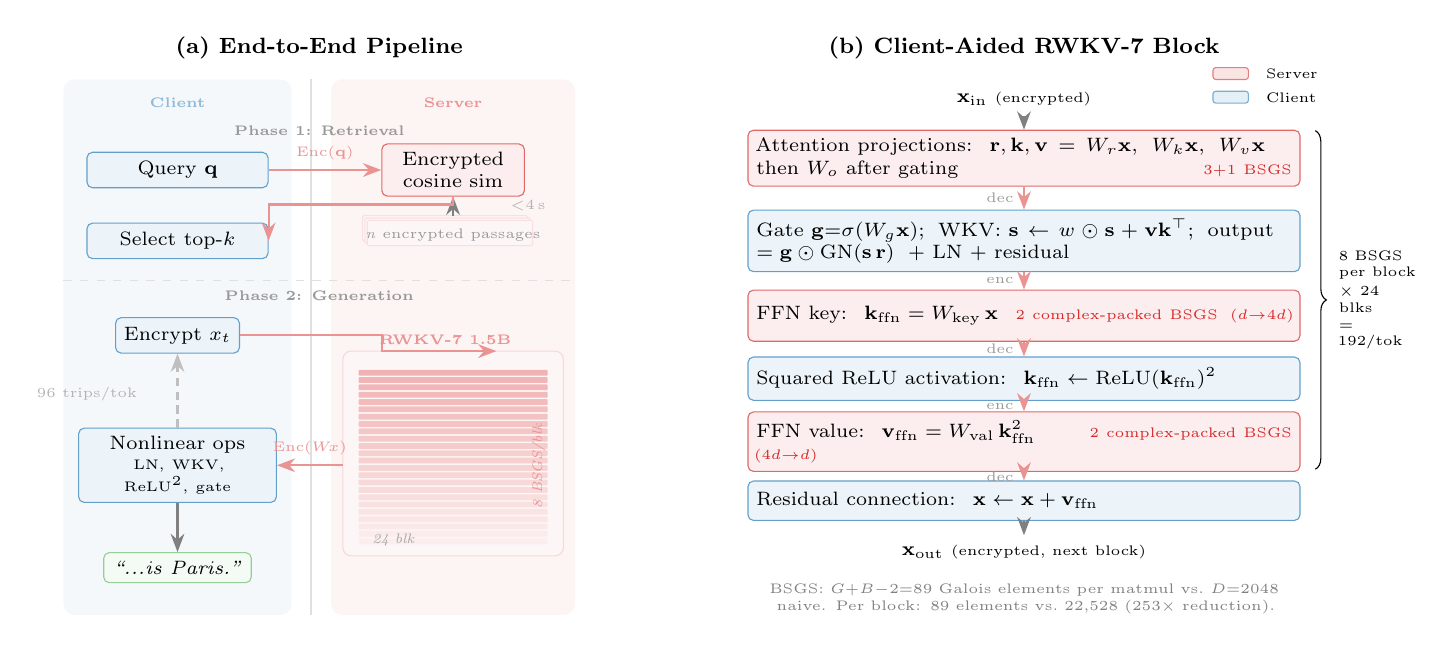
\begin{tikzpicture}[
    font=\scriptsize,
    >=Stealth,
    cop/.style={draw=ourmethod!70, fill=ourmethod!8, rounded corners=2pt,
        inner sep=3pt, minimum height=0.45cm},
    sop/.style={draw=aenoise!70, fill=aenoise!8, rounded corners=2pt,
        inner sep=3pt, minimum height=0.45cm},
    arr/.style={->, thick, black!50},
    ctarr/.style={->, thick, aenoise!50},
]
% ===== Panel (a): E2E Pipeline =====
\begin{scope}
\node[font=\footnotesize\bfseries] at (3.25, 7.1) {(a) End-to-End Pipeline};

% Background regions
\fill[ourmethod!5, rounded corners=4pt] (0, -0.1) rectangle (2.9, 6.7);
\fill[aenoise!5, rounded corners=4pt] (3.4, -0.1) rectangle (6.5, 6.7);
\draw[black!12, thick] (3.15, -0.1) -- (3.15, 6.7);
\node[font=\tiny\bfseries, ourmethod!50] at (1.45, 6.4) {\textsc{Client}};
\node[font=\tiny\bfseries, aenoise!50] at (4.95, 6.4) {\textsc{Server}};

% Phase 1: Retrieval
\node[font=\tiny\bfseries, black!40] at (3.25, 6.05) {\textsc{Phase 1: Retrieval}};

\node[cop, minimum width=2.3cm] (q) at (1.45, 5.55) {Query $\mathbf{q}$};
\node[sop, text width=1.6cm, align=center] (sim) at (4.95, 5.55) {Encrypted\\cosine sim};
\draw[ctarr] (q) -- (sim) node[midway, above, font=\tiny] {$\mathrm{Enc}(\mathbf{q})$};

% Corpus (stacked documents)
\foreach \i in {0,1,2} {
  \fill[aenoise!4, draw=aenoise!15, rounded corners=0.5pt]
      (3.8+\i*0.03, 4.65-\i*0.03) rectangle ++(2.1, 0.32);
}
\node[font=\tiny, black!40] at (4.95, 4.73) {\textit{n} encrypted passages};
\draw[arr] (4.95, 4.97) -- (sim);

\node[cop, minimum width=2.3cm] (sel) at (1.45, 4.65) {Select top-$k$};
\draw[ctarr] (sim.south) -- ++(0,-0.1) -| (sel.east);
\node[font=\tiny, black!30] at (5.9, 5.1) {$<$4\,s};

% Phase 2: Generation
\draw[black!12, dashed] (0, 4.15) -- (6.5, 4.15);
\node[font=\tiny\bfseries, black!40] at (3.25, 3.95) {\textsc{Phase 2: Generation}};

\node[cop] (tok) at (1.45, 3.45) {Encrypt $x_t$};

% RWKV tower (24 stacked blocks with gradient)
\fill[aenoise!4, draw=aenoise!18, rounded corners=3pt] (3.55, 0.65) rectangle (6.35, 3.25);
\node[font=\tiny\bfseries, aenoise!50] at (4.85, 3.4) {RWKV-7 1.5B};
\foreach \i in {0,...,23} {
  \pgfmathsetmacro{\yy}{0.8+\i*0.093}
  \pgfmathsetmacro{\sh}{8+\i*1.2}
  \fill[aenoise!\sh, rounded corners=0.3pt]
      (3.75, \yy) rectangle (6.15, \yy+0.073);
}
\node[font=\tiny, black!35, anchor=west] at (3.8, 0.85) {\textit{24 blk}};
\node[font=\tiny, aenoise!50, rotate=90, anchor=south] at (6.25, 1.8) {\textit{8 BSGS/blk}};

\draw[ctarr] (tok.east) -- ++(1.8,0) |- (5.5, 3.25);

% Client nonlinear operations
\node[cop, text width=2.3cm, align=center] (nl) at (1.45, 1.8) {Nonlinear ops\\[-1pt]{\tiny LN, WKV, ReLU$^2$, gate}};
\draw[ctarr] (3.55, 1.8) -- (nl) node[midway, above, font=\tiny] {$\mathrm{Enc}(W\!x)$};

% Generation loop arrow
\draw[arr, densely dashed, black!25] (nl.north) -- ++(0, 0.55) -| (tok);
\node[font=\tiny, black!30] at (0.3, 2.7) {96 trips/tok};

% Output text
\node[draw=randproj!50, fill=randproj!5, rounded corners=2pt, inner sep=3pt]
    (out) at (1.45, 0.5) {\textit{``...is Paris.''}};
\draw[arr] (nl) -- (out);
\end{scope}

% ===== Panel (b): Single RWKV-7 Block =====
\begin{scope}[shift={(8.2, 0)}]
\node[font=\footnotesize\bfseries] at (4.0, 7.1) {(b) Client-Aided RWKV-7 Block};

% Legend
\fill[aenoise!12, draw=aenoise!60, rounded corners=1pt] (6.4, 6.7) rectangle ++(0.45, 0.15);
\node[font=\tiny, anchor=west] at (6.95, 6.77) {Server};
\fill[ourmethod!12, draw=ourmethod!60, rounded corners=1pt] (6.4, 6.4) rectangle ++(0.45, 0.15);
\node[font=\tiny, anchor=west] at (6.95, 6.47) {Client};

% Input
\node (xin) at (4.0, 6.45) {$\mathbf{x}_\mathrm{in}$ {\tiny(encrypted)}};

% S1: Time-mix projections
\node[sop, text width=6.8cm, align=left, minimum height=0.7cm] (s1) at (4.0, 5.7) {
  Attention projections:\;
  $\mathbf{r}, \mathbf{k}, \mathbf{v} = W_{r}\mathbf{x},\; W_{k}\mathbf{x},\; W_{v}\mathbf{x}$\quad
  then $W_o$ after gating
  \hfill {\tiny\textcolor{aenoise}{3{+}1 BSGS}}
};

% C1: WKV state + gating
\node[cop, text width=6.8cm, align=left, minimum height=0.75cm] (c1) at (4.0, 4.65) {
  Gate $\mathbf{g}{=}\sigma(W_g\mathbf{x})$;\;
  WKV: $\mathbf{s} \leftarrow w \odot \mathbf{s} + \mathbf{v}\mathbf{k}^\top$;\;
  output $= \mathbf{g} \odot \mathrm{GN}(\mathbf{s}\,\mathbf{r})$\; + LN + residual
};

% S2: FFN key
\node[sop, text width=6.8cm, align=left, minimum height=0.65cm] (s2) at (4.0, 3.7) {
  FFN key:\;
  $\mathbf{k}_\text{ffn} = W_\text{key}\,\mathbf{x}$
  \hfill {\tiny\textcolor{aenoise}{2 complex-packed BSGS\; ($d{\to}4d$)}}
};

% C2: ReLU squared
\node[cop, text width=6.8cm, align=left, minimum height=0.55cm] (c2) at (4.0, 2.9) {
  Squared ReLU activation:\;
  $\mathbf{k}_\text{ffn} \leftarrow \mathrm{ReLU}(\mathbf{k}_\text{ffn})^2$
};

% S3: FFN value
\node[sop, text width=6.8cm, align=left, minimum height=0.65cm] (s3) at (4.0, 2.1) {
  FFN value:\;
  $\mathbf{v}_\text{ffn} = W_\text{val}\,\mathbf{k}_\text{ffn}^2$
  \hfill {\tiny\textcolor{aenoise}{2 complex-packed BSGS\; ($4d{\to}d$)}}
};

% C3: Residual
\node[cop, text width=6.8cm, align=left, minimum height=0.5cm] (c3) at (4.0, 1.35) {
  Residual connection:\;
  $\mathbf{x} \leftarrow \mathbf{x} + \mathbf{v}_\text{ffn}$
};

% Output
\node (xout) at (4.0, 0.7) {$\mathbf{x}_\mathrm{out}$ {\tiny(encrypted, next block)}};

% Vertical arrows with enc/dec labels
\draw[arr] (xin) -- (s1);
\draw[ctarr] (s1) -- (c1) node[midway, left, font=\tiny, black!40] {dec};
\draw[ctarr] (c1) -- (s2) node[midway, left, font=\tiny, black!40] {enc};
\draw[ctarr] (s2) -- (c2) node[midway, left, font=\tiny, black!40] {dec};
\draw[ctarr] (c2) -- (s3) node[midway, left, font=\tiny, black!40] {enc};
\draw[ctarr] (s3) -- (c3) node[midway, left, font=\tiny, black!40] {dec};
\draw[arr] (c3) -- (xout);

% Right brace: total BSGS calls
\draw[decorate, decoration={brace, amplitude=4pt}]
    (7.7, 6.05) -- (7.7, 1.75)
    node[midway, right=5pt, font=\tiny, align=left, text width=1.0cm] {8 BSGS\\per block\\[1pt]$\times$ 24 blks\\= 192/tok};

% Bottom: BSGS rotation count
\node[font=\tiny, black!50, text width=7.5cm, align=center] at (4.0, 0.1) {
  BSGS: $G{+}B{-}2{=}89$ Galois elements per matmul vs.\ $D{=}2048$ naive.
  Per block: 89 elements vs.\ 22{,}528 (253$\times$ reduction).
};
\end{scope}
\end{tikzpicture}
\caption{\textbf{(a)}~Two-phase client-server protocol. Phase~1 retrieves relevant passages via encrypted cosine similarity over the document corpus. Phase~2 generates tokens by running RWKV-7 blocks on the server (BSGS-accelerated diagonal matrix-vector products) with client-side nonlinear operations, requiring 96 round-trips per generated token. The server operates exclusively on CKKS ciphertexts.
\textbf{(b)}~Anatomy of a single RWKV-7 block. The server performs 8 BSGS matrix-vector products per block (4 attention, 2 complex-packed FFN key, 2 complex-packed FFN value); the client handles all nonlinear operations (layer normalization, WKV recurrence, gating, squared ReLU). Data is encrypted and decrypted at each boundary crossing, yielding 4 round-trips per block.}
\label{fig:overview}
\end{figure*}

Our contributions:

\begin{enumerate}
    \item \textbf{Complex Packing}: Encoding two dimensions per CKKS slot using real and imaginary components. Queries packed as conjugates yield inner products in the real part. This halves ciphertext count compared to vertical packing.

    \item \textbf{Encrypted SSM Inference}: Multi-layer RWKV inference under CKKS with CT-CT squaring and no intermediate decryption. BSGS diagonal acceleration extends fully encrypted inference to 19 blocks at $d{=}2048$ (perfect correlation) and 24 blocks with CKKS bootstrap (correlation 0.99999). Magnitude-controlled normalization and client-side head completion support 65{,}536 tokens.

    \item \textbf{Encrypted Similarity Joins}: CT-CT similarity computation where both queries and documents are encrypted, with SIMD batching and GPU acceleration for throughput.

    \item \textbf{Hyperbolic Embeddings}: The Lorentz hyperboloid model provides FHE-compatible hyperbolic geometry via the bilinear form $\langle q, d \rangle_\mathcal{L} = -q_0 d_0 + \sum_{i>0} q_i d_i$.

    \item \textbf{FHE-Sim}: Predicts encrypted similarity accuracy from embedding statistics using $\rho_{\text{FHE}} = \rho_{\text{compression}} \times \rho_{\text{noise}}$, validated at 1.7\% mean error (Appendix~\ref{appendix:fhesim}).
\end{enumerate}

% ============================================================
\section{Background}

\subsection{CKKS Homomorphic Encryption}

The CKKS scheme~\cite{cheon2017homomorphic} encrypts vectors of real numbers with approximate arithmetic:
\begin{equation}
    \text{sim}(\mathbf{x}, \mathbf{y}) = \mathbf{x}^\top \mathbf{y} \approx \text{Dec}(\text{Enc}(\mathbf{x}) \cdot \mathbf{y})
\end{equation}

Ciphertext size and operation latency depend on the polynomial modulus degree $N$:
\begin{itemize}
    \item $N=8192$: 326KB ciphertexts, $\sim$31ms per similarity
    \item $N=4096$: 79KB ciphertexts, $\sim$4ms per similarity
\end{itemize}

\subsection{Problem Formulation}

Given embeddings $\{\mathbf{x}_i\}_{i=1}^M$ where $\mathbf{x}_i \in \mathbb{R}^{D}$, we seek a compression function $f: \mathbb{R}^{D} \rightarrow \mathbb{R}^{d}$ (with $d \ll D$) maximizing:
\begin{equation}
    \rho\Big(\{\mathbf{x}_i^\top \mathbf{x}_j\}, \{\text{FHE}(f(\mathbf{x}_i), f(\mathbf{x}_j))\}\Big)
\end{equation}
where $\rho$ is Pearson correlation and FHE$(\cdot,\cdot)$ computes similarity under encryption.

\subsection{Threat Model and Protocol}

We consider two settings differing in what the server observes:

\textbf{PT-CT.} The server holds plaintext document embeddings $\{d_i\}$. A client encrypts a query $\text{Enc}(q)$; the server computes ciphertext-plaintext products $\text{Enc}(q) \cdot d_i$ and returns encrypted scores. The server learns nothing about query content.

\textbf{CT-CT (Encrypted Similarity Joins).} Both query and document embeddings are encrypted. The server holds $\{\text{Enc}(d_i)\}$ and receives $\text{Enc}(q)$. Using CKKS ciphertext-ciphertext multiplication, the server computes $\text{Enc}(q \cdot d_i)$ without observing either embedding. This provides mutual privacy: neither party reveals their data to the server.

Access pattern hiding (which documents were retrieved) requires ORAM techniques orthogonal to this work.

\textbf{CKKS Parameters.} Retrieval experiments use $N=4096$ with coefficient modulus $[40, 20, 40]$ bits and scale $2^{20}$, achieving $\sim$128-bit security with 79KB ciphertexts and $\sim$4ms per similarity. Generation experiments (Section~\ref{sec:ssm}) use $N=32768$ with scale $2^{40}$ to provide sufficient multiplicative depth for CT-CT operations.

\textbf{Per-user access control.} In multi-user deployments, different users may be authorized for different corpus subsets. We address this using additive noise cancellation within the existing CKKS scheme, requiring no additional cryptographic primitive. At ingestion, passages are classified by PII content into sensitivity classes (financial, personal, temporal, organizational). Per-class random noise $\mathbf{n}_c$ with $\|\mathbf{n}_c\| \gg \|\mathbf{e}_j\|$ is added to each restricted embedding before encryption: $\mathrm{Enc}(\mathbf{e}_j + \mathbf{n}_c)$. Each user receives correction ciphertexts: $\mathrm{Enc}(-\mathbf{n}_c)$ for authorized classes, $\mathrm{Enc}(\mathbf{r})$ (random) for unauthorized classes. These are indistinguishable under CKKS IND-CPA security. The server applies all corrections via homomorphic addition (zero multiplicative levels consumed); authorized passages are restored to $\mathrm{Enc}(\mathbf{e}_j)$ while unauthorized passages remain noise-dominated. Details and experiments in Appendix~\ref{appendix:access_control}.

\textbf{Generation threat model.} In the client-aided protocol (Section~\ref{sec:bsgs}), the server performs matrix-vector products on CKKS ciphertexts and never observes any plaintext. The client decrypts intermediate hidden states to apply non-linear operations, then re-encrypts before sending the next projection. Since RWKV-7 weights are public, intermediate activations do not leak model information; the security goal is purely data privacy. The server's view consists entirely of CKKS ciphertexts and Galois-rotated ciphertexts, indistinguishable from random under the RLWE assumption. GAZELLE~\cite{juvekar2018gazelle} and CrypTFlow2~\cite{rathee2020cryptflow2} use the same client-server split. The per-token communication pattern is fixed: exactly 96 round-trips of identically sized ciphertexts, with the same sequence of operations regardless of input content. Client-side element-wise computation (${\sim}\mu$s on $d{=}2048$ vectors) is negligible relative to CKKS encryption and network transfer (${\sim}$ms), limiting observable timing variation. Output length (number of tokens generated) is not hidden.

\textbf{Out of scope.} We do not hide access patterns, result set size, query volume, or output length. These require additional techniques (ORAM, differential privacy) orthogonal to our contribution. The client holds the secret key and decrypts similarity scores to select top-k; server-side encrypted ranking is out of scope.

% ============================================================
\section{Characterizing FHE Accuracy}
\label{sec:fhe_accuracy}

Two relationships govern FHE accuracy for similarity search.

\subsection{Noise Scaling}

\begin{lemma}[FHE Noise Scaling]
\label{thm:noise}
For CKKS dot product of $d$-dimensional vectors, the noise standard deviation satisfies:
\begin{equation}
    \sigma_\epsilon(d) = c \cdot \sqrt{d}
\end{equation}
where $c$ is a constant depending on encryption parameters.
\end{lemma}

\textbf{Proof sketch}: The dot product $z = \sum_{i=1}^d x_i y_i$ sums $d$ terms. Each term has independent noise. By variance additivity: $\text{Var}(z_\epsilon) = d \cdot \sigma_{\text{term}}^2$, giving $\sigma_\epsilon \propto \sqrt{d}$.

\textbf{Empirical validation}: We measure noise across dimensions 8--256 using TenSEAL CKKS (Table~\ref{tab:noise}). The ratio $\sigma_\epsilon/\sqrt{d}$ is constant ($c \approx 0.0028$), confirming Lemma~\ref{thm:noise}.

\begin{table}[ht]
\centering
\caption{CKKS noise scales as $\sqrt{d}$ ($N=4096$, scale $2^{20}$). Measured correlation $\rho$ on random unit vectors.}
\label{tab:noise}
\begin{tabular}{lcccc}
\toprule
\textbf{Dim} & $\sigma_\epsilon$ & $\sqrt{d}$ & $c = \sigma/\sqrt{d}$ & $\rho$ (measured) \\
\midrule
8 & 0.0089 & 2.83 & 0.0031 & 99.98\% \\
16 & 0.0106 & 4.00 & 0.0026 & 99.94\% \\
32 & 0.0150 & 5.66 & 0.0027 & 99.69\% \\
64 & 0.0219 & 8.00 & 0.0027 & 98.51\% \\
128 & 0.0301 & 11.3 & 0.0027 & 95.22\% \\
256 & 0.0464 & 16.0 & 0.0029 & 85.45\% \\
\bottomrule
\end{tabular}
\end{table}

\subsection{The Prediction Formula}

\begin{lemma}[FHE Similarity Correlation Bound]
Let $\sigma_z$ be the standard deviation of latent pairwise similarities and $\sigma_\epsilon$ be the CKKS noise standard deviation. The Pearson correlation between true and encrypted similarities is bounded by:
\begin{equation}
    \rho \leq \frac{\sigma_z}{\sqrt{\sigma_z^2 + \sigma_\epsilon^2}}
\end{equation}
Equality holds when the CKKS error is modeled as independent, mean-zero additive noise.
\end{lemma}

This bound connects embedding geometry to FHE performance. However, the SNR bound alone is insufficient; it does not account for information lost during compression.

\begin{corollary}[FHE Prediction Formula]
FHE correlation is the product of compression quality and noise tolerance:
\begin{equation}
    \rho_{\text{FHE}} = \rho_{\text{compression}} \times \rho_{\text{noise}}
\end{equation}
where $\rho_{\text{compression}} = \text{corr}(\text{original\_sims}, \text{compressed\_sims})$ measures how well SVD preserves similarity structure, and $\rho_{\text{noise}} = \sigma_z / \sqrt{\sigma_z^2 + \sigma_\epsilon^2}$ is the SNR bound.
\end{corollary}

\textbf{Validation}: We validate the formula by comparing predicted correlation to actual CKKS correlation measured with TenSEAL across dimensions 16--64 (Appendix~\ref{appendix:fhesim}). The prediction formula requires only $\rho_{\text{compression}}$ (measurable without FHE) and CKKS parameters, so embedding-dimension configurations can be evaluated without expensive FHE benchmarks (500--8,000$\times$ faster than running actual encryption).

% === THE TWO LAWS FIGURE ===
\begin{figure*}[t]
\centering
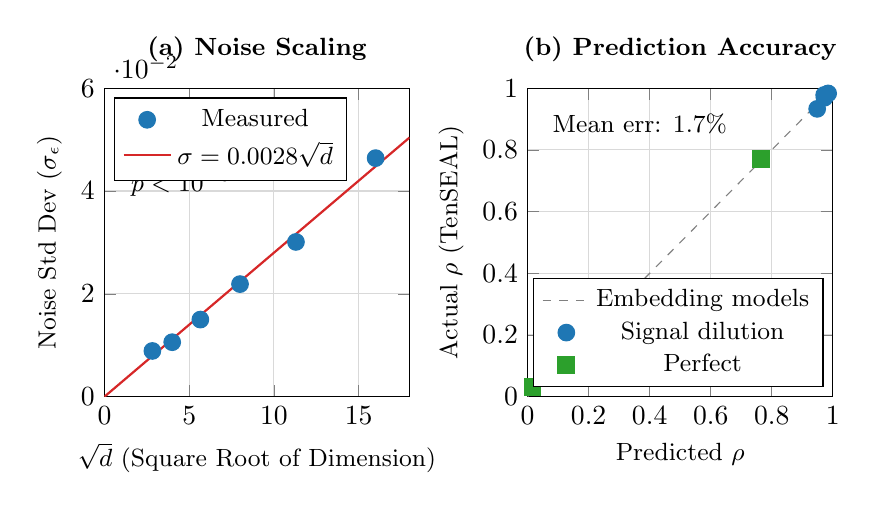
\begin{tikzpicture}
% Left plot: Noise Scaling Law
\begin{axis}[
    name=left,
    width=0.45\textwidth,
    height=5.5cm,
    xlabel={$\sqrt{d}$ (Square Root of Dimension)},
    ylabel={Noise Std Dev ($\sigma_\epsilon$)},
    xlabel style={font=\small},
    ylabel style={font=\small},
    xmin=0, xmax=18,
    ymin=0, ymax=0.06,
    legend pos=north west,
    legend style={font=\small},
    grid=major,
    grid style={gray!30},
    title={(a) Noise Scaling},
    title style={font=\small\bfseries},
]
% Data points
\addplot[only marks, mark=*, color=ourmethod, mark size=3pt] coordinates {
    (2.83, 0.0089) (4.00, 0.0106) (5.66, 0.0150) (8.00, 0.0219) (11.3, 0.0301) (16.0, 0.0464)
};
% Fit line
\addplot[color=aenoise, thick, domain=0:18] {0.0028*x};
\legend{Measured, $\sigma = 0.0028\sqrt{d}$}
% R^2 annotation
\node[anchor=south west, font=\small] at (axis cs:1,0.045) {$R^2 = 0.98$};
\node[anchor=south west, font=\small] at (axis cs:1,0.037) {$p < 10^{-6}$};
\end{axis}

% Right plot: Prediction Accuracy
\begin{axis}[
    name=right,
    at={(left.east)},
    anchor=west,
    xshift=1.5cm,
    width=0.45\textwidth,
    height=5.5cm,
    xlabel={Predicted $\rho$},
    ylabel={Actual $\rho$ (TenSEAL)},
    xlabel style={font=\small},
    ylabel style={font=\small},
    xmin=0, xmax=1.0,
    ymin=0, ymax=1.0,
    legend pos=south east,
    legend style={font=\small},
    grid=major,
    grid style={gray!30},
    title={(b) Prediction Accuracy},
    title style={font=\small\bfseries},
]
% Perfect prediction line
\addplot[color=gray, dashed, domain=0:1.0] {x};
% Data points: (predicted, actual)
\addplot[only marks, mark=*, color=ourmethod, mark size=3pt] coordinates {
    (0.949, 0.933) (0.973, 0.969) (0.985, 0.983) (0.972, 0.978)
};
\addplot[only marks, mark=square*, color=randproj, mark size=3pt] coordinates {
    (0.764, 0.771) (0.288, 0.290) (0.016, 0.031)
};
\legend{Embedding models, Signal dilution, Perfect}
% Annotations
\node[anchor=north west, font=\small] at (axis cs:0.05,0.95) {Mean err: 1.7\%};
\end{axis}
\end{tikzpicture}
\caption{\textbf{FHE-Sim.} (a) Noise Scaling ($N=4096$): CKKS noise scales as $\sigma_\epsilon = c\sqrt{d}$ with $R^2 = 0.98$ (variance additivity). (b) Prediction accuracy across embedding models and signal corruption levels (1.7\% mean error over 396 configs; Appendix~\ref{appendix:fhesim}).}
\label{fig:validation}
\end{figure*}

\subsection{Contrastive Failure}

The prediction formula explains why contrastive compression methods fail under FHE: they produce embeddings where $\rho_{\text{compression}} \approx 0$.

\begin{proposition}[InfoNCE Similarity Concentration]
\label{thm:contrastive}
Let $f^*$ minimize the InfoNCE loss
\begin{equation}
    \mathcal{L}_{\text{NCE}} = -\log \frac{\exp(z_i \cdot z_{j^+} / \tau)}{\sum_k \exp(z_i \cdot z_k / \tau)}
\end{equation}
with $K \to \infty$ negatives in $d$ dimensions. Then:
\begin{enumerate}
    \item \textbf{Alignment.} Positive pairs satisfy $f^*(x) \cdot f^*(x^+) = 1$.
    \item \textbf{Concentration.} For independently drawn negative pairs, $f^*(x_i) \cdot f^*(x_j)$ has mean $0$ and variance $1/d$, concentrating in $[-O(1/\sqrt{d}),\; O(1/\sqrt{d})]$ with high probability.
\end{enumerate}
\end{proposition}

\textbf{Proof.} Part (1): Wang \& Isola~\cite{wang2020understanding} decompose InfoNCE into alignment and uniformity terms. The alignment term is minimized when $f^*(x) = f^*(x^+)$, giving $f^*(x) \cdot f^*(x^+) = 1$ on the unit sphere. Part (2): the uniformity term is minimized when the output distribution of $f^*$ is uniform on $S^{d-1}$. For independently drawn $x_i, x_j$, $f^*(x_i)$ and $f^*(x_j)$ are independent uniform on $S^{d-1}$, so their dot product has mean $0$ and variance $1/d$ with sub-Gaussian tails.

\begin{proposition}[FHE Consequence]
\label{prop:infonce_fhe}
At the InfoNCE optimum, all negative similarities concentrate in a band of width $O(1/\sqrt{d})$ around zero. The encoded similarity variance is $\sigma_z^2 \approx 1/d$. Combined with CKKS noise $\sigma_\epsilon = c\sqrt{d}$:
\begin{equation}
    \rho_{\text{noise}} = \frac{1}{\sqrt{1 + c^2 d^2}}
\end{equation}
which decreases with dimension. At $d = 64$, the band is $\pm 0.125$: a pair with original similarity $0.3$ and one at $0.7$ both map to values near $0$, collapsing the continuous similarity range. Empirically, $\rho_{\text{compression}} \approx 0.01$ (Table~\ref{tab:infonce}); the concentration destroys correlation with original similarities.
\end{proposition}

High uniformity alone does not cause FHE failure. BERT embeddings have $U = 0.70$ yet achieve 97\% FHE correlation because $\rho_{\text{compression}} = 0.99$. InfoNCE fails because it removes similarity structure, not because it increases uniformity.

\begin{table}[ht]
\centering
\caption{InfoNCE removes similarity structure ($\rho_{\text{compression}} \approx 0$).}
\label{tab:infonce}
\begin{tabular}{lcccc}
\toprule
\textbf{Method} & \textbf{Uniformity} & $\rho_{\text{comp}}$ & $\rho_{\text{noise}}$ & \textbf{FHE} \\
\midrule
SVD (64-d) & 0.64 & 0.99 & 0.98 & 97\% \\
BERT (high-U) & 0.70 & 0.99 & 0.98 & 97\% \\
\midrule
InfoNCE & 0.99 & 0.01 & 0.98 & 1\% \\
Random & 0.99 & 0.01 & 0.98 & 1\% \\
\bottomrule
\end{tabular}
\end{table}

The formula $\rho_{\text{FHE}} = \rho_{\text{compression}} \times \rho_{\text{noise}}$ explains both successes and failures: InfoNCE has high $\rho_{\text{noise}}$ but near-zero $\rho_{\text{compression}}$, yielding near-zero FHE correlation.

% ============================================================
\section{FHE-Sim}

FHE-Sim predicts whether a given embedding model's similarity structure survives compression and CKKS encryption. It does not model general FHE computation; it specifically captures the interaction between embedding geometry, dimensionality reduction, and encryption noise for dot-product similarity search.

\textbf{Failure mode detection}: FHE-Sim identifies failure modes via $\rho_{\text{compression}}$:
\begin{itemize}
    \item \textbf{Latent collapse} ($\sigma_z < 0.01$): Autoencoder failure
    \item \textbf{Similarity destruction} ($\rho_{\text{comp}} < 0.5$): Contrastive/random failure
\end{itemize}

\begin{algorithm}[ht]
\caption{FHE-Sim: Predict FHE Accuracy}
\begin{algorithmic}[1]
\STATE \textbf{Input}: Embeddings $X$, poly\_modulus\_degree $N$, target dim $d$
\STATE Compress: $Z = \text{SVD}_d(X)$
\STATE Compute $\rho_{\text{comp}} = \text{corr}(X_i \cdot X_j, Z_i \cdot Z_j)$
\STATE Compute $\sigma_z = \text{std}(Z_i \cdot Z_j)$
\STATE Lookup noise constant: $c = f(N)$
\STATE Compute $\rho_{\text{noise}} = \sigma_z / \sqrt{\sigma_z^2 + c^2 d}$
\STATE \textbf{Output}: $\rho_{\text{comp}} \times \rho_{\text{noise}}$, compatibility
\end{algorithmic}
\end{algorithm}

\begin{table}[ht]
\centering
\caption{FHE-Sim predictions for SVD vs.\ InfoNCE (2 models, $d{=}64$, $N{=}4096$).}
\label{tab:predictions}
\begin{tabular}{llccc}
\toprule
\textbf{Model} & \textbf{Method} & \textbf{Pred.} & \textbf{Actual} & \textbf{Err.} \\
\midrule
OpenAI & SVD & 100\% & 97.8\% & 2.2\% \\
OpenAI & InfoNCE & 13.2\% & 16.1\% & 2.9\% \\
BERT & SVD & 100\% & 97.2\% & 2.8\% \\
BERT & InfoNCE & 16.1\% & 19.4\% & 3.3\% \\
\midrule
\multicolumn{4}{l}{\textbf{Mean error}} & \textbf{2.8\%} \\
\bottomrule
\end{tabular}
\end{table}

\subsection{Simulation Mode}

FHE-Sim can also simulate CKKS outputs by adding calibrated Gaussian noise:
\begin{equation}
    \text{sim}_{\text{FHE}}(x, y) = \langle x, y \rangle + \mathcal{N}(0, c\sqrt{d})
\end{equation}

For $N=4096$, simulated correlation matches TenSEAL CKKS within 0.5\% (500--8,000$\times$ compute time reduction vs. running actual encryption~\cite{benaissa2021tenseal}). For $N=8192$ with scale $2^{40}$, CKKS noise is negligible ($\sim$1e-7) and simulation is unnecessary.

% ============================================================
\section{Complex Packing}

CKKS encodes vectors into polynomial slots, where each slot holds a complex number $a + bi$. Standard vertical packing uses only the real component, leaving imaginary components unused.

\medskip\noindent
\begin{minipage}{\columnwidth}
\centering
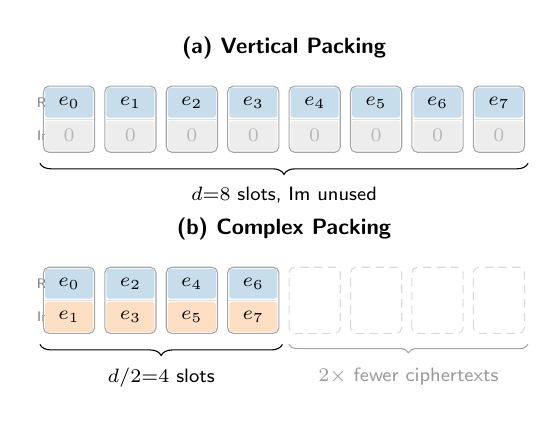
\begin{tikzpicture}[
    font=\sffamily\scriptsize,
]

\def\slotw{0.65}
\def\sloth{0.38}
\def\slotsep{0.78}

% ===== (a) Vertical Packing =====
\node[font=\sffamily\footnotesize\bfseries, anchor=south] at (2.73, 3.5) {(a) Vertical Packing};

\node[font=\sffamily\tiny, text=black!50, anchor=east] at (-0.08, 3.07) {Re};
\node[font=\sffamily\tiny, text=black!50, anchor=east] at (-0.08, 2.65) {Im};

\foreach \i in {0,...,7} {
    \pgfmathsetmacro{\x}{\i*\slotsep}
    % Outer slot
    \draw[black!35, rounded corners=2pt, line width=0.4pt]
        (\x-0.325, 2.44) rectangle ++(0.65, 0.84);
    % Re half (blue)
    \fill[ourmethod!25, rounded corners=1pt]
        (\x-0.305, 2.88) rectangle ++(0.61, 0.38);
    \node at (\x, 3.07) {$e_{\i}$};
    % Divider
    \draw[black!12, line width=0.3pt] (\x-0.305, 2.86) -- ++(0.61, 0);
    % Im half (gray, wasted)
    \fill[black!7, rounded corners=1pt]
        (\x-0.305, 2.46) rectangle ++(0.61, 0.38);
    \node[text=black!28] at (\x, 2.65) {$0$};
}

\draw[decorate, decoration={brace, amplitude=4pt, mirror}]
    (-0.37, 2.3) -- (5.83, 2.3)
    node[midway, below=5pt, font=\sffamily\scriptsize] {$d{=}8$ slots, Im unused};

% ===== (b) Complex Packing =====
\node[font=\sffamily\footnotesize\bfseries, anchor=south] at (2.73, 1.2) {(b) Complex Packing};

\node[font=\sffamily\tiny, text=black!50, anchor=east] at (-0.08, 0.77) {Re};
\node[font=\sffamily\tiny, text=black!50, anchor=east] at (-0.08, 0.35) {Im};

\foreach \i/\re/\im in {0/0/1, 1/2/3, 2/4/5, 3/6/7} {
    \pgfmathsetmacro{\x}{\i*\slotsep}
    \draw[black!35, rounded corners=2pt, line width=0.4pt]
        (\x-0.325, 0.14) rectangle ++(0.65, 0.84);
    % Re (blue)
    \fill[ourmethod!25, rounded corners=1pt]
        (\x-0.305, 0.58) rectangle ++(0.61, 0.38);
    \node at (\x, 0.77) {$e_{\re}$};
    \draw[black!12, line width=0.3pt] (\x-0.305, 0.56) -- ++(0.61, 0);
    % Im (orange, utilized)
    \fill[pca!25, rounded corners=1pt]
        (\x-0.305, 0.16) rectangle ++(0.61, 0.38);
    \node at (\x, 0.35) {$e_{\im}$};
}

\foreach \i in {4,...,7} {
    \pgfmathsetmacro{\x}{\i*\slotsep}
    \draw[black!15, rounded corners=2pt, densely dashed, line width=0.4pt]
        (\x-0.325, 0.14) rectangle ++(0.65, 0.84);
}

\draw[decorate, decoration={brace, amplitude=4pt, mirror}]
    (-0.37, 0.0) -- (2.71, 0.0)
    node[midway, below=5pt, font=\sffamily\scriptsize] {$d/2{=}4$ slots};
\draw[decorate, decoration={brace, amplitude=3pt, mirror}, black!35]
    (2.79, 0.0) -- (5.83, 0.0)
    node[midway, below=5pt, font=\sffamily\scriptsize, text=black!40] {$2\times$ fewer ciphertexts};

\end{tikzpicture}
\vspace{2pt}
\captionof{figure}{CKKS slot utilization for $d{=}8$. \textbf{(a)}~Vertical packing stores one real value per slot, leaving imaginary components unused. \textbf{(b)}~Complex packing maps consecutive pairs as $e_{2j} + i\mkern1mu e_{2j+1}$, fully utilizing each slot and halving ciphertext count.}
\label{fig:complex_packing}
\end{minipage}
\medskip

\subsection{Packing Scheme}

We pack two consecutive embedding dimensions into each slot:
\begin{equation}
    \text{slot}_j = e_{2j} + i \cdot e_{2j+1}
\end{equation}
For a $d$-dimensional embedding, this requires $d/2$ slots instead of $d$.

Queries are packed as conjugates:
\begin{equation}
    \text{slot}_j^{(q)} = q_{2j} - i \cdot q_{2j+1}
\end{equation}

\subsection{Inner Product Recovery}

The ciphertext-plaintext product yields:
\begin{align}
    (e_r + i \cdot e_i)(q_r - i \cdot q_i) &= (e_r q_r + e_i q_i) \\
    &\quad + i(e_i q_r - e_r q_i)
\end{align}
The real part equals $e_r q_r + e_i q_i$, the contribution of two dimensions to the inner product. Summing real parts across slots gives the full inner product.

Complex packing is mathematically identical to vertical packing but halves ciphertext count. Compared to standard approaches using 768-dimensional embeddings (e.g., BERT-base) with vertical packing, our 64d complex-packed representation uses $768 / 32 = 24\times$ fewer ciphertexts.

% ============================================================
\section{Hyperbolic Embeddings}

Euclidean space may not be optimal for embedding hierarchical or tree-structured data. Hyperbolic geometry provides exponentially more volume at a given radius, better matching the growth rate of hierarchical structures~\cite{nickel2017poincare}.

\subsection{The Lorentz Model}

We use the Lorentz (hyperboloid) model $\mathcal{L}^n = \{x \in \mathbb{R}^{n+1} : \langle x, x \rangle_\mathcal{L} = -1, x_0 > 0\}$ where the Lorentz inner product is:
\begin{equation}
    \langle x, y \rangle_\mathcal{L} = -x_0 y_0 + \sum_{i=1}^{n} x_i y_i
\end{equation}

For FHE, this reduces to a standard dot product with a sign flip on the first component; no transcendental functions are needed.

\subsection{FHE-Compatible Similarity}

For points on the hyperboloid, the hyperbolic distance is $d_\mathcal{L}(x,y) = \text{arcosh}(-\langle x, y \rangle_\mathcal{L})$. Since $\text{arcosh}$ is monotonic, ranking by $-\langle x, y \rangle_\mathcal{L}$ preserves the distance ordering.

Under CKKS with complex packing, we encode:
\begin{align}
    d_j &= d_{2j} + i \cdot d_{2j+1} \\
    q_j &= \begin{cases}
        -q_0 + i \cdot q_1 & j = 0 \text{ (time component negated)} \\
        q_{2j} - i \cdot q_{2j+1} & j > 0 \text{ (conjugate)}
    \end{cases}
\end{align}

The real part of $\sum_j q_j \cdot d_j$ yields $-q_0 d_0 + \sum_{i>0} q_i d_i = \langle q, d \rangle_\mathcal{L}$.

\subsection{Euclidean to Hyperbolic Projection}

Given Euclidean embeddings $e \in \mathbb{R}^d$, we project to the hyperboloid via:
\begin{equation}
    x = \left(\sqrt{1 + \|W e\|^2}, \; W e\right)
\end{equation}
where $W \in \mathbb{R}^{n \times d}$ is learned. The time component $x_0 = \sqrt{1 + \|x_{1:n}\|^2}$ ensures $\langle x, x \rangle_\mathcal{L} = -1$.

On MS MARCO, Lorentz hyperbolic embeddings achieve 90.5\% R@10 vs 88.0\% Euclidean (+2.5\%), with identical FHE operations. Beyond accuracy, the Lorentz model enables complex packing (Eq.~9--10): pairing coordinates as real and imaginary parts halves slot usage per document, doubling SIMD throughput (e.g.\ 124 vs 62 documents per ciphertext at $N{=}8192$). This $2\times$ packing is used throughout retrieval and generation (Section~\ref{sec:bsgs}).

% ============================================================
\section{Experiments}
\label{sec:experiments}

\subsection{Setup}

\textbf{Retrieval benchmark.} MS MARCO passage retrieval: 1,214 queries, 10,001 documents. Strict train/test split: queries 0--799 for training projections, 800+ for evaluation. All reported metrics are on the test set.

\textbf{Embeddings.} Qwen3-Embedding-0.6B (1024d, MRL-trained), OpenAI text-embedding-3-large (1536d), all-MiniLM-L6-v2 (384d).

\textbf{FHE implementations.} CPU: TenSEAL/Pyfhel with $N=4096$. GPU: PhantomFHE~\cite{phantomfhe2024} on NVIDIA RTX 3090 and A100 80GB ($N$ up to 32768). We implemented CKKS bootstrapping for PhantomFHE (CoeffToSlot/EvalMod/SlotToCoeff with direct RNS scalar multiplication) and extended its Python bindings with a \texttt{cuDoubleComplex} type caster for complex packing.

\textbf{Baselines.} SVD (no centering), random projection, learned linear projections with InfoNCE and ranking distillation losses.

\subsection{Similarity Preservation}

Before evaluating retrieval, we verify that compression preserves similarity structure. Using OpenAI \texttt{text-embedding-3-large} (1536d), we measure Pearson correlation between original and FHE-computed similarities.

\begin{table}[h]
\centering
\caption{Similarity correlation ($N$=4096). Higher is better.}
\label{tab:main}
\begin{tabular}{lcccc}
\toprule
\textbf{Dim} & \textbf{RP} & \textbf{SVD} & \textbf{Learned} & \textbf{MLP} \\
\midrule
32 & 82.3\% & 94.7\% & 95.7\% & 94.2\% \\
64 & 86.8\% & 96.8\% & 96.9\% & 96.2\% \\
128 & 91.7\% & 97.4\% & 97.2\% & --- \\
\bottomrule
\end{tabular}
\end{table}

SVD without centering matches learned methods. Standard PCA implementations center data before projection; for unit-normalized embeddings, this can degrade similarity structure (effect varies by embedding characteristics):

\begin{table}[h]
\centering
\caption{Effect of centering on similarity correlation (OpenAI, 64d). The gap ranges from 7--24\% depending on embedding characteristics.}
\label{tab:centering}
\begin{tabular}{lc}
\toprule
\textbf{Method} & \textbf{Correlation} \\
\midrule
\texttt{sklearn.PCA} (centered) & 73.2\% \\
SVD / TruncatedSVD (no centering) & \textbf{97.1\%} \\
\bottomrule
\end{tabular}
\end{table}

\subsection{Recall@k}

We evaluate retrieval quality using Recall@k on the MS MARCO test set.

\begin{table}[h]
\centering
\caption{Recall@k comparison (MS MARCO test set, 64d).}
\label{tab:recall}
\begin{tabular}{lcc}
\toprule
\textbf{Method} & \textbf{R@10} & \textbf{R@100} \\
\midrule
MS MARCO 384d + SVD 64d & 65.2\% & 89.1\% \\
MS MARCO 384d + learned 64d & 65.2\% & --- \\
\midrule
Qwen3 MRL truncate 64d & 92.3\% & 99.5\% \\
Qwen3 distilled 64d & 94.8\% & 99.7\% \\
\textbf{Qwen3 combined 64d} & \textbf{95.0\%} & \textbf{99.7\%} \\
\midrule
Qwen3 MRL truncate 128d & 96.2\% & 99.8\% \\
Qwen3 full 1024d & 98.2\% & 100\% \\
\bottomrule
\end{tabular}
\end{table}

Qwen3-Embedding is trained with Matryoshka Representation Learning (MRL)~\cite{kusupati2022matryoshka}, so truncating to the first 64 of 1024 dimensions yields a valid embedding without any learned projection. Moving from generic embeddings (65.2\%) to MRL truncation (92.3\%) yields the largest gain. Ranking distillation (Appendix~\ref{appendix:rankingkd}) contributes an additional 2.7 percentage points.

\subsection{CT-CT: Encrypted Similarity Joins}

In CT-CT mode, both query and document embeddings are encrypted. The server computes similarities via ciphertext-ciphertext multiplication without observing either party's data.

\textbf{SIMD Batching.} Complex packing yields 33 slots per 64d Lorentz embedding. With $N=8192$ providing 4096 slots, we pack $\lfloor 4096/33 \rfloor = 124$ documents per ciphertext. A single ciphertext-ciphertext multiplication computes 124 similarities in parallel.

\begin{table}[ht]
\centering
\caption{CT-PT vs CT-CT performance with GPU acceleration and SIMD batching.}
\label{tab:ctct}
\begin{tabular}{lcccc}
\toprule
\textbf{Documents} & \textbf{CT-PT} & \textbf{CT-CT} & \textbf{Per-doc} & \textbf{Ranking} \\
\midrule
1,000 & 17ms & 16ms & 16$\mu$s & 10/10 \\
10,000 & 143ms & 131ms & 14$\mu$s & 10/10 \\
50,000 & 835ms & 630ms & 13$\mu$s & 10/10 \\
\bottomrule
\end{tabular}
\end{table}

CT-CT achieves 13--16$\mu$s per document at 64 dimensions, giving sub-second retrieval over 50,000 documents. CT-CT is faster than CT-PT (0.76--0.94$\times$) because pre-encrypted documents avoid repeated plaintext encoding overhead during query processing. The ``Ranking'' column verifies FHE correctness: encrypted rankings match plaintext rankings exactly.

\subsection{Latency and Throughput}

\begin{table}[ht]
\centering
\caption{PT-CT latency comparison (CPU, TenSEAL). Compression allows a smaller polynomial modulus.}
\label{tab:latency}
\begin{tabular}{lccc}
\toprule
\textbf{Configuration} & \textbf{Latency} & \textbf{Size} & \textbf{QPS} \\
\midrule
1536-d ($N$=8192) & 31.4ms & 326KB & 32 \\
1536-d ($N$=4096) & 8.6ms & 79KB & 116 \\
\midrule
64-d ($N$=4096) & 4.0ms & 79KB & 252 \\
\bottomrule
\end{tabular}
\end{table}

Dimensionality reduction provides 7.9$\times$ speedup over production parameters on CPU. For CT-CT with GPU acceleration, see Table~\ref{tab:ctct}.

\begin{figure}[ht]
\centering
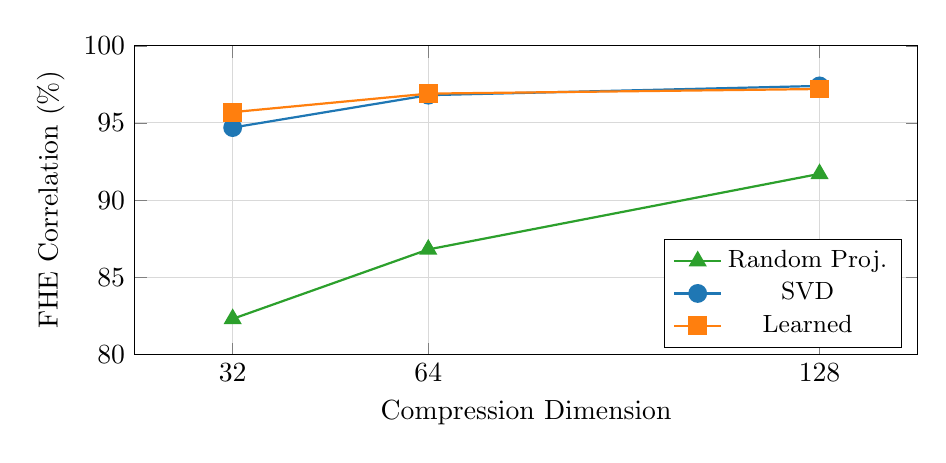
\begin{tikzpicture}
\begin{axis}[
    width=0.95\columnwidth,
    height=5.5cm,
    xlabel={Compression Dimension},
    ylabel={FHE Correlation (\%)},
    xmin=16, xmax=144,
    ymin=80, ymax=100,
    xtick={32, 64, 128},
    legend style={at={(0.98,0.02)}, anchor=south east, font=\small},
    grid=major,
    grid style={gray!30},
]
% Random Projection
\addplot[mark=triangle*, color=randproj, thick, mark size=3pt] coordinates {
    (32, 82.3) (64, 86.8) (128, 91.7)
};
% SVD
\addplot[mark=*, color=ourmethod, thick, mark size=3pt] coordinates {
    (32, 94.7) (64, 96.8) (128, 97.4)
};
% Learned
\addplot[mark=square*, color=pca, thick, mark size=3pt] coordinates {
    (32, 95.7) (64, 96.9) (128, 97.2)
};
\legend{Random Proj., SVD, Learned}
\end{axis}
\end{tikzpicture}
\caption{Similarity correlation vs dimension. SVD preserves 97\% correlation at 64d. For retrieval metrics (R@10), see Table~\ref{tab:recall}.}
\label{fig:dim_accuracy}
\end{figure}

% ============================================================
\section{State Space Models for FHE Generation}
\label{sec:ssm}

While retrieval under FHE is addressed by the techniques above, \textit{generation} under FHE has remained impractical. Transformer architectures require softmax attention: $\text{softmax}(QK^\top/\sqrt{d})V$, where $\text{softmax}(x)_i = e^{x_i}/\sum_j e^{x_j}$. Both exponentials and divisions are prohibitively expensive under CKKS, and the $O(n^2)$ attention complexity compounds the cost.

State space models (SSMs) offer a fundamentally different computational structure. Linear recurrent architectures like RWKV~\cite{peng2025rwkv7} and Mamba~\cite{gu2023mamba} use only:
\begin{enumerate}
    \item Matrix-vector multiplications
    \item Element-wise products
    \item Gating activations (sigmoid, exp)
\end{enumerate}

While certain gating activations (sigmoid, exp) require polynomial approximation, the dominant feedforward nonlinearity in RWKV (squared activation) can be computed exactly via ciphertext--ciphertext multiplication.

\textbf{Polynomial approximation of SSM nonlinearities.} We verify that all RWKV-7 gating functions (sigmoid, tanh, exponential decay $e^{-e^{-0.5} \cdot \sigma(w)}$) are polynomial-friendly. Table~\ref{tab:poly_stress} shows Chebyshev polynomial approximation across 15 diverse prompts and 20 tokens each, replacing all nonlinearities simultaneously during full 1.5B model inference ($d{=}2048$, 24 blocks). At degree 19, every generated token matches exact arithmetic.

\begin{table}[ht]
\centering
\small
\caption{Polynomial approximation of RWKV-7 nonlinearities (1.5B model, 24 blocks, 15 prompts $\times$ 20 tokens). Chebyshev polynomials replace sigmoid, tanh, and exponential decay simultaneously.}
\label{tab:poly_stress}
\begin{tabular}{rccc}
\toprule
\textbf{Degree} & \textbf{Prompts} & \textbf{Tokens} & \textbf{Match Rate} \\
\midrule
11 & 11/15 & 268/300 & 89.3\% \\
13 & 12/15 & 271/300 & 90.3\% \\
15 & 12/15 & 271/300 & 90.3\% \\
\textbf{19} & \textbf{15/15} & \textbf{300/300} & \textbf{100\%} \\
\bottomrule
\end{tabular}
\end{table}

Table~\ref{tab:poly_ckks} evaluates sigmoid polynomials on CKKS ciphertexts (A100, $N{=}32768$, $L_0{=}20$, 40-bit primes), using binary powering for depth-efficient power basis construction. Degree 11--13 consumes only 5 multiplicative levels with sub-percent error, comparable to a single BSGS matmul call.

\begin{table}[ht]
\centering
\small
\caption{Sigmoid polynomial evaluation under CKKS (A100, 100 test points on $[-6, 6]$). Levels = multiplicative depth consumed.}
\label{tab:poly_ckks}
\begin{tabular}{rcccc}
\toprule
\textbf{Degree} & \textbf{Levels} & \textbf{Time} & \textbf{Max Err} & \textbf{Corr.} \\
\midrule
7 & 4 & 35\,ms & $2.2 \times 10^{-2}$ & 0.9995 \\
11 & 5 & 53\,ms & $4.9 \times 10^{-3}$ & 0.99998 \\
\textbf{13} & \textbf{5} & \textbf{62\,ms} & $\mathbf{2.3 \times 10^{-3}}$ & \textbf{0.99999} \\
\bottomrule
\end{tabular}
\end{table}

By contrast, transformer softmax requires normalization by $\sum_j e^{x_j}$, which involves $1/\sqrt{\cdot}$ over encrypted values. Profiling RWKV-7's normalization layers (LayerNorm, GroupNorm) reveals input variance spanning 5 orders of magnitude ($[6 \times 10^{-4},\; 2 \times 10^4]$), making polynomial approximation of $1/\sqrt{\cdot}$ infeasible at any practical degree. SSM gating functions operate on bounded, well-conditioned inputs ($[-8, 8]$ for sigmoid/tanh); transformer normalization does not.

\subsection{Fully Encrypted Inference}

We run RWKV-7 (1.5B) token prediction under CKKS, using trained model weights. No intermediate decryptions; logits are decrypted only at the output. Unless otherwise noted, all configurations in this section achieve exact functional agreement with plaintext inference (correlation 1.0, identical predicted tokens).

The single-block pipeline consists of: embedding lookup (plaintext), encryption of the hidden state, FFN key projection (CT-PT), ciphertext--ciphertext squaring activation (CT-CT), FFN value projection (CT-PT), head projection (CT-PT), and decryption of final logits followed by argmax. For numerical stability under CKKS, we apply column-wise variance normalization to weights and scale embeddings by a constant factor.

The squaring operation corresponds to the dominant nonlinear component of RWKV's squared-ReLU feedforward block. We evaluate configurations up to 1024 hidden dimensions and 2048 intermediate dimensions using CKKS with poly modulus degree 32768 and scale $2^{40}$.

\begin{table}[ht]
\centering
\caption{Fully encrypted RWKV inference with $x^2$ activation (RTX 3090).}
\label{tab:fhe_rwkv}
\begin{tabular}{lcc}
\toprule
\textbf{Hidden$\times$FFN$\times$Vocab} & \textbf{Activation} & \textbf{Time} \\
\midrule
64$\times$128$\times$32 & $x^2$ & 7.6s \\
128$\times$256$\times$64 & $x^2$ & 27.7s \\
256$\times$512$\times$64 & $x^2$ & 96.3s \\
512$\times$1024$\times$64 & $x^2$ & 355.8s \\
1024$\times$2048$\times$64 & $x^2$ & 1401.8s \\
\bottomrule
\end{tabular}
\end{table}

Runtimes scale with the number of encrypted dot products; the nonlinear activation is not the dominant cost.

\subsection{Multi-Layer FHE Inference}

We extend to multi-layer inference by chaining $N$ feedforward blocks under a single encryption, with no intermediate decryption. Each block consumes 3 multiplicative levels (key projection, squaring, value projection), plus 1 for the final head projection, giving a total depth of $3N + 1$.

Block 0 operates on a packed ciphertext (full hidden vector in one ciphertext) using \texttt{ct\_pt\_dot} with rotate-and-sum for the key projection. The output is a \textit{list} of ciphertexts (one scalar per FFN dimension). Subsequent blocks operate on this list representation, using \texttt{ct\_pt\_weighted\_sum} for all projections. This avoids costly repacking while preserving the exact same FHE primitives.

The modulus chain $[60, 40 \times d, 60]$ with one special prime provides $d$ multiplicative levels. At $N=32768$, security constraints allow up to $d=19$ levels (880 bits total modulus), supporting $\lfloor(19-1)/3\rfloor = 6$ chained blocks. We evaluate configurations from 2 to 6 blocks using weights from consecutive RWKV-7 layers:

\begin{table}[ht]
\centering
\small
\setlength{\tabcolsep}{4pt}
\caption{Multi-layer FHE RWKV inference (RTX 3090, no intermediate decryption). Each block: key projection, $x^2$ activation, value projection. $\dagger$~magnitude-controlled normalization.}
\label{tab:fhe_rwkv_multi}
\begin{tabular}{lcccc}
\toprule
\textbf{Config} & \textbf{Blocks} & \textbf{Depth} & \textbf{Time} & \textbf{Mag-Ctrl} \\
\midrule
64$\times$128$\times$32 & 2 & 7/9 & 28.4s & \\
128$\times$256$\times$64 & 2 & 7/9 & 142.0s & \\
64$\times$128$\times$32 & 3 & 10/11 & 75.1s & \\
128$\times$256$\times$64 & 3 & 10/11 & 186.9s & \\
\midrule
64$\times$128$\times$32 & 4 & 13/14 & 63.2s & $\dagger$ \\
64$\times$128$\times$32 & 5 & 16/17 & 83.1s & $\dagger$ \\
64$\times$128$\times$32 & 6 & 19/20 & 104.6s & $\dagger$ \\
128$\times$256$\times$64 & 4 & 13/14 & 321.6s & $\dagger$ \\
\bottomrule
\end{tabular}
\end{table}

\textbf{Magnitude-controlled normalization.} Without normalization, cascaded squaring causes exponential magnitude growth: $|h|_\text{max} \approx 10^{6}$ after 2 blocks, $10^{14}$ after 3, and $10^{32}$ after 4, causing CKKS precision loss (correlation $\approx 0.04$ at 4 blocks). We solve this by absorbing per-block scaling factors into $W_\text{val}$: after computing plaintext magnitudes on one calibration input, we set $W_\text{val}^{(b)} \leftarrow W_\text{val}^{(b)} \cdot (\alpha / |h^{(b)}|_\infty)$ for a target magnitude $\alpha = 10$. Since \texttt{argmax} is scale-invariant, the predicted token is identical. This adds zero extra multiplicative depth: the scaling is folded into existing plaintext multiplications. With magnitude control, 4--6 blocks all match plaintext, extending the practical depth from 10 to 19 levels within the same $N=32768$ parameter set.

\textbf{Residual connections.} Ciphertext-level skip connections for blocks 1+ are achieved via \texttt{mod\_switch\_to\_next} (level alignment, 0 extra depth) and \texttt{set\_scale} (scale matching), followed by ciphertext addition. Both 2- and 3-block configurations with residuals match plaintext at zero additional multiplicative cost.

\textbf{Autoregressive generation.} Multi-token generation: each token step encrypts the embedding, runs multi-layer FHE inference, decrypts logits, and applies argmax. The client (who holds the secret key) selects each token; the server never observes any plaintext token. With 2-block inference, 5 consecutive tokens match plaintext (191.0s total, RTX 3090); with 3 blocks, 3 tokens match (134.0s total).

\textbf{Time-mixing under FHE.} RWKV's time-mixing path computes $\sigma(r) \odot (k \cdot v)$ projected through $W_o$, where $\sigma$ is the sigmoid gate. We approximate $\sigma(x) \approx 0.25x + 0.5$ (linear sigmoid), consuming 0 extra multiplicative levels since it decomposes into a plaintext scaling and addition. Level alignment requires care: $r$ and $k$ are both at 1 rescale after their respective \texttt{ct\_pt\_dot} projections, so $r \cdot k$ (CT-CT) produces a result at 2 rescales. We then align $v$ via \texttt{mod\_switch\_to\_next} (0 extra depth) before computing $(r \cdot k) \cdot v$ at 3 rescales. One block of time-mixing + FFN uses 7 multiplicative levels (4 for time-mix, 3 for FFN, 24.5s on RTX 3090). Multi-block time-mixing requires magnitude control for the combined path.

\subsection{Scaling to Full Vocabulary}

The experiments above use reduced vocabulary sizes (32--64 tokens) because the head projection $h \mapsto W_\text{head} h$ requires one encrypted weighted sum per vocabulary token. At the full RWKV-7 vocabulary of 65{,}536 tokens, computing 65{,}536 encrypted weighted sums is prohibitively expensive.

\textbf{Client-side head completion.} The head projection need not be computed under FHE. Since the client already decrypts all logits to apply argmax, the server can simply return the encrypted hidden state $h$. The client decrypts $h$ ($d_\text{embed}$ values), applies $W_\text{head} \in \mathbb{R}^{d_\text{embed} \times V}$ in plaintext, and takes argmax. This introduces no approximation, supports any vocabulary size, and saves one multiplicative level (depth $3N$ instead of $3N+1$ for $N$ blocks). The security model is unchanged: the server never observes any plaintext, and the client already receives the logit vector in all protocols.

\textbf{Batched FHE computation.} At full model dimensions ($d_\text{embed}=2048$, $d_\text{ffn}=8192$), holding all intermediate ciphertexts simultaneously exceeds GPU memory. We process FFN dimensions in batches of 1024, fusing key projection and squaring for each dimension (avoiding storing both $\text{ct}_k$ and $\text{ct}_{k^2}$ simultaneously) and accumulating partial value projections across batches via ciphertext addition. Peak memory drops from $O(2 \times d_\text{ffn})$ to $O(b + d_\text{embed})$ ciphertexts.

\begin{table}[ht]
\centering
\small
\setlength{\tabcolsep}{4pt}
\caption{Full-vocabulary FHE inference ($V{=}65{,}536$, RTX 3090) with client-side head. $\dagger$~magnitude-controlled.}
\label{tab:fhe_fullscale}
\begin{tabular}{lccc}
\toprule
\textbf{Hidden$\times$FFN$\times$Vocab} & \textbf{Blocks} & \textbf{Depth} & \textbf{Time} \\
\midrule
64$\times$128$\times$65536 & 1 & 3/5 & 5.9s \\
128$\times$2048$\times$65536 & 1 & 3/5 & 177.7s \\
1024$\times$2048$\times$65536 & 1 & 3/5 & 1381.0s \\
1024$\times$2048$\times$65536$^\dagger$ & 2 & 6/8 & 4096.9s \\
2048$\times$8192$\times$65536 & 1 & 3/5 & 10863.4s \\
\bottomrule
\end{tabular}
\end{table}

Client-side head completion at $V=65{,}536$ takes $<$1s in plaintext, avoiding 65{,}536 encrypted weighted sums. The 1024$\times$2048 configuration completes one token in 23 minutes on a single consumer GPU (RTX 3090); since FFN dimensions are processed independently, the workload parallelizes linearly.

\subsection{Encrypted RAG Pipeline}

We combine encrypted retrieval (Section~\ref{sec:experiments}) with encrypted generation into a single private RAG pipeline.

\textbf{Protocol.} The pipeline uses two CKKS contexts optimized for each phase:
\begin{enumerate}
    \item \textbf{Encrypted retrieval} ($N=8192$, complex packing): The client encrypts the query embedding; the server computes batched similarity scores against all documents via SIMD packing (124 docs per ciphertext). In CT-PT mode, documents remain as plaintexts; in CT-CT mode, documents are pre-encrypted, providing full bilateral encryption. The client decrypts scores and selects the top document.
    \item \textbf{Encrypted generation}: At small dimensions (top rows of Table~\ref{tab:e2e}), the server runs fully encrypted multi-block inference with no intermediate decryptions. At full scale (bottom rows), the client-aided BSGS protocol (Section~\ref{sec:bsgs}) is used, where the server performs matrix-vector products on encrypted data and the client handles non-linear operations between projections.
\end{enumerate}

The two phases share no cryptographic state; the only bridge is the client's plaintext decision of which document was retrieved. In both cases, the server never observes any plaintext query, document, or generated token.

\begin{table}[ht]
\centering
\small
\setlength{\tabcolsep}{3pt}
\caption{Encrypted RAG pipeline. Top: fully encrypted at small dimensions. Bottom: client-aided BSGS at full scale (A100). All generated tokens match plaintext (correlation 1.0).}
\label{tab:e2e}
\begin{tabular}{lccccc}
\toprule
\textbf{Config} & \textbf{Blk} & \textbf{Docs} & \textbf{Mode} & \textbf{Ret.} & \textbf{Gen.} \\
\midrule
64$\times$128$\times$32 & 2 & 100 & CT-PT & 48ms & 82.1s \\
64$\times$128$\times$32 & 3 & 200 & CT-PT & 50ms & 145.7s \\
128$\times$256$\times$64 & 2 & 100 & CT-PT & 76ms & 336.6s \\
64$\times$128$\times$32 & 2 & 100 & CT-CT & 69ms & 96.6s \\
\midrule
2048$\times$8192$\times$65k & 24 & 100 & CT-PT & 1.0s & 429s/tok \\
2048$\times$8192$\times$65k & 24 & 100 & CT-CT & 1.0s & 429s/tok \\
1024$\times$4096$\times$65k$^\dagger$ & 24 & 100 & CT-PT & 1.0s & 23s/tok \\
\bottomrule
\end{tabular}
\vspace{2pt}

{\footnotesize $^\dagger$0.4B model, $N{=}8192$, CPU-offloaded diagonals. 50 queries (30 SQuAD + 20 MS-MARCO), all 50/50 tokens match plaintext.}
\end{table}

Retrieval latency is dominated by a single batched ciphertext multiplication ($<$100\,ms at small dimensions; $<$4\,s at full scale). In CT-CT mode both query and documents are encrypted, providing bilateral privacy.

The full-scale rows use client-aided BSGS (Section~\ref{sec:bsgs}). On 100 SQuAD passages with 3 queries at $d{=}2048$, CT-PT and CT-CT both achieve 3/3 gold recall at rank~1, and every generated token matches plaintext RWKV-7 (correlation 1.0). Token-matching means QA metrics under FHE equal the plaintext model's. At $d{=}1024$ (0.4B) with CPU-offloaded pre-encoded diagonals, we scale to 50 queries across both datasets: 30/30 SQuAD and 20/20 MS-MARCO queries produce FHE tokens identical to plaintext (correlation 1.0), with 23\,s/token on the A100. Retrieval recall (16/30 SQuAD, 19/20 MS-MARCO at R@1) reflects the embedding model's capacity at 100 passages rather than the encryption pipeline. Neither RWKV-7 1.5B nor comparably sized models (e.g.\ Qwen2.5-1.5B~\cite{qwen2025qwen25}, MMLU 45--46) are tuned for extractive QA; these scores reflect the base model's capacity at this scale.

\subsection{Client-Aided Generation with BSGS Acceleration}
\label{sec:bsgs}

The fully encrypted approach (Tables~\ref{tab:fhe_rwkv}--\ref{tab:fhe_fullscale}) computes all operations under a single encryption without intermediate decryption, but is limited to shallow depth by the CKKS modulus chain. To scale to the full 24-block RWKV-7 (1.5B parameters, $d=2048$, $d_\text{ffn}=8192$), we adopt a \emph{client-aided protocol} combined with the baby-step giant-step (BSGS) diagonal method for matrix-vector products.

\textbf{Protocol.} Each RWKV block is partitioned between server and client:
\begin{enumerate}
    \item \textbf{Server (FHE):} computes the six large matrix-vector products ($r$, $k$, $v$, $o$ projections at $d \times d$; FFN key at $d \times d_\text{ffn}$; FFN value at $d_\text{ffn} \times d$) using CKKS-encrypted inputs.
    \item \textbf{Client (plaintext):} decrypts server outputs and performs all non-linear operations: LayerNorm, GroupNorm, sigmoid gating, WKV state update, and ReLU$^2$ activation.
\end{enumerate}
The client re-encrypts each intermediate result before sending it back for the next server projection. Per block, this requires 4 client-server round-trips ($r{,}k{,}v$ jointly, then $o$, then FFN key, then FFN value), giving 96 round-trips per token across 24 blocks. The server never observes any plaintext hidden state.

\textbf{Computation split.} The server holds the six projection matrices per block (${\sim}2.7$\,GB for 24 blocks in float16) and performs all $O(d^2)$ and $O(d \cdot d_\text{ffn})$ matrix-vector products under FHE. The client holds the embedding table, output head, and per-block normalization/gating vectors (${\sim}550$\,MB), performing only $O(d)$ element-wise operations (LayerNorm, sigmoid, WKV update, ReLU$^2$) that take $<$0.01s per block. The client offloads the expensive linear algebra to a GPU server while keeping all data encrypted, following the outsourced computation model of GAZELLE~\cite{juvekar2018gazelle}. Since the model weights are public (RWKV-7 is Apache-licensed), the security goal is data privacy, not model privacy: the server must not learn the client's query, retrieved documents, or generated text.

\textbf{BSGS diagonal method.} For $y = Wx$ where $W \in \mathbb{R}^{d \times d}$, the standard approach computes each output element independently via a rotate-and-sum dot product, requiring $d \cdot \lceil\log_2 d\rceil$ rotations per projection. The diagonal method~\cite{halevi2014algorithms} decomposes $W$ into $d$ diagonals $\delta_k[j] = W[j, (j{+}k) \bmod d]$ and computes $y = \sum_{k=0}^{d-1} \text{rotate}(x, k) \odot \delta_k$, encoding all $d$ output elements in a single ciphertext via SIMD packing. Baby-step giant-step factoring writes $k = gG + b$ with $G = \lceil\sqrt{d}\rceil$, $B = \lceil d/G \rceil$, reducing the rotation count to $G + B - 2$ (identity rotations require no key). At $d = 2048$: $G = 46$, $B = 45$, giving $G{+}B{-}2 = 89$ rotations per projection versus $2048 \times 11 = 22{,}528$ in the naive approach, a 253$\times$ reduction.

\textbf{Complex packing.} For the FFN key projection ($d \to d_\text{ffn} = 4d$), we split the output into 4 chunks of $d$ elements each. Since the input is real-valued, we pack two weight chunks as real and imaginary parts of complex-valued diagonals, computing two output chunks per BSGS call, reducing the cost from 4 to 2 calls. For the FFN value projection ($d_\text{ffn} \to d$), the 4 input chunks are paired using the conjugate trick: we encrypt $\text{Enc}(x_0 + i x_1)$ and encode diagonals as $(\delta_0 - i\delta_1)$ so that $\text{Re}(\text{BSGS}(\cdot)) = M_0 x_0 + M_1 x_1$, again reducing 4 real BSGS calls to 2 complex ones. Both directions share baby-step rotations within each pair, and partial results accumulate in plaintext.

Each BSGS call consumes exactly 1 multiplicative level (one \texttt{rescale\_to\_next}), independent of $d$, versus $d$ rescales in the naive per-element approach. This eliminates the depth bottleneck that previously limited inference to a single block at full model dimensions.

\begin{table}[ht]
\centering
\small
\setlength{\tabcolsep}{3pt}
\caption{Client-aided BSGS generation across model sizes, CKKS parameters, and GPUs. All configurations produce identical tokens under FHE and plaintext (3 tokens, 24 blocks). The 1.5B generates ``\emph{is Paris.}'' on the RTX 3090; both models generate ``\emph{Paris}'' on the A100. $^\dagger$CPU-offloaded plaintexts with FFN value complex packing (8 BSGS calls/block).}
\label{tab:bsgs_generation}
\resizebox{\columnwidth}{!}{%
\begin{tabular}{llcccc}
\toprule
\textbf{Model ($d$)} & \textbf{GPU} & \textbf{$N$} & \textbf{Server/blk} & \textbf{Client/blk} & \textbf{Per token} \\
\midrule
1.5B (2048) & RTX 3090 & 32768 & 20.6s & $<$0.01s & 494s (8.2 min) \\
1.5B (2048) & A100 80GB & 16384 & 14.1s & $<$0.01s & 338s (5.6 min) \\
1.5B (2048) & A100 80GB & 8192 & 8.9s & $<$0.01s & 213s (3.6 min) \\
1.5B (2048) & A100 80GB$^\dagger$ & 8192 & 3.1s & $<$0.01s & 79s (1.3 min) \\
0.4B (1024) & A100 80GB & 16384 & 6.6s & $<$0.01s & 160s (2.7 min) \\
0.4B (1024) & A100 80GB & 8192 & 4.0s & $<$0.01s & 96s (1.6 min) \\
0.4B (1024) & A100 80GB$^\dagger$ & 8192 & 0.8s & $<$0.01s & 19s \\
\bottomrule
\end{tabular}%
}
\end{table}

Client computation is negligible ($<$0.1\% of total time). Each of the 24 blocks requires 8 BSGS calls (4 for attention projections, 2 complex-packed for FFN key, 2 complex-packed for FFN value). Pre-encoding all diagonal plaintexts on the CPU and streaming them to the GPU via a persistent staging buffer eliminates per-call device allocation overhead, reducing per-block server time from 8.9s to 3.1s on the A100 at $N{=}8{,}192$. The per-token latency scales linearly with block count and is independent of vocabulary size (client-side head completion).

\textbf{Parameter tuning.} In the client-aided protocol, each BSGS matmul consumes exactly one multiplicative level; the client decrypts and re-encrypts between projections, resetting the level budget. This means only $L_0{=}3$ working levels are needed (down from 5), and the polynomial degree can be reduced from $N{=}16{,}384$ to $N{=}8{,}192$ while remaining within the HE Standard's 128-bit security bound ($\log_2 Q = 216 \leq 218$ for $N{=}8{,}192$). The smaller polynomial degree halves the NTT size, reducing per-block latency from 14.1s to 8.9s for the 1.5B model and from 6.6s to 4.0s for the 0.4B model. Combining both optimizations (smaller model and smaller $N$) yields a 3.5$\times$ overall speedup.

Compared to the fully encrypted single-block approach (Table~\ref{tab:fhe_fullscale}), the full 24-block model under the client-aided protocol completes one token (19--494s) in less time than a single naive block at the same dimensions (10{,}863s). The per-block speedup arises from BSGS rotation reduction ($89$ vs ${\sim}22{,}500$) and client-side non-linearities. The cost is 96 client-server round-trips per token, each transmitting one ciphertext (${\sim}4$\,MB at $N{=}32768$, ${\sim}1$\,MB at $N{=}8192$).

\textbf{Full-scale RAG.} Combining BSGS-accelerated generation with the encrypted retrieval pipeline (Section~\ref{sec:experiments}), we run retrieval + generation on SQuAD v2 and MS-MARCO. At $d{=}2048$ (100 passages, 3 queries, 3 tokens each), both CT-PT and CT-CT retrieval achieve 3/3 gold recall at rank~1 (429\,s/token). At $d{=}1024$ with CPU-offloaded pre-encoded diagonals (23\,s/token), we scale to 50 queries: 30 SQuAD and 20 MS-MARCO, each generating 3 tokens. All 50/50 queries produce FHE tokens identical to plaintext (correlation 1.0). Retrieval R@1 is 16/30 on SQuAD and 19/20 on MS-MARCO (Table~\ref{tab:e2e}).

\textbf{Token count.} Since FHE tokens match plaintext exactly (correlation 1.0), the useful token count is limited by the model, not the encryption. At $d{=}2048$ (full 1.5B, 24 blocks), greedy decoding on 10 diverse prompts produces 30 coherent tokens each with no token-level degeneration; sentence-level repetition (common in greedy LM decoding) is the only quality-limiting factor.

\textbf{Retrieval mode ablation.} To verify that encryption introduces no ranking errors, we run retrieval-only benchmarks with 100 passages and 10 queries in three modes: plaintext (no encryption), CT-PT (encrypted query, plaintext documents), and CT-CT (both encrypted). Table~\ref{tab:retrieval_ablation} confirms that all three modes produce identical rankings on both datasets.

\begin{table}[ht]
\centering
\small
\setlength{\tabcolsep}{4pt}
\caption{Retrieval mode ablation (100 passages, 10 queries). All three modes produce identical rankings. Latency is per-query with GPU-accelerated SIMD batching.}
\label{tab:retrieval_ablation}
\begin{tabular}{llcccc}
\toprule
\textbf{Dataset} & \textbf{Mode} & \textbf{R@1} & \textbf{R@5} & \textbf{R@10} & \textbf{ms/q} \\
\midrule
SQuAD & Plaintext & 80\% & 90\% & 100\% & 1.3 \\
SQuAD & CT-PT & 80\% & 90\% & 100\% & 1.8 \\
SQuAD & CT-CT & 80\% & 90\% & 100\% & 1.4 \\
\midrule
MS-MARCO & Plaintext & 90\% & 90\% & 100\% & 0.2 \\
MS-MARCO & CT-PT & 90\% & 90\% & 100\% & 1.6 \\
MS-MARCO & CT-CT & 90\% & 90\% & 100\% & 1.4 \\
\bottomrule
\end{tabular}
\end{table}

Retrieval adds $<$4\,s per query. Generation latency (429--443\,s/token at $N{=}16{,}384$) is dominated by per-block BSGS computation (Table~\ref{tab:bsgs_generation}); retrieval overhead is $<$1\%.

\textbf{Plaintext prefill.} In the RAG setting, the client already possesses the retrieved passage (having decrypted the retrieval result). Rather than feeding only a short seed token into FHE generation, the client can construct a full prompt (``Context: \{passage\}$\backslash$nQuestion: \{query\}$\backslash$nAnswer:'') and process it entirely through the plaintext RWKV forward pass, building up the recurrent WKV state across all 24 blocks. Only the answer generation phase then runs under FHE. Since RWKV's state is a fixed-size $d_\text{head} \times d_\text{head}$ matrix per head per block (independent of sequence length), the full context is compressed into the state; the server receives an encrypted state that encodes the complete passage without knowing its content. Prefilling a 200-token prompt takes $<$2\,s in plaintext on CPU, after which the model generates short answers (``Paris'' for a factual question) in as few as 1--3 FHE tokens (19--494\,s per token depending on GPU and model size). This amortizes context processing to $<$10\% of total latency even at the fastest configuration.

\subsection{Fully Encrypted BSGS Inference with Bootstrap}
\label{sec:fully_encrypted_bsgs}

The client-aided protocol (Section~\ref{sec:bsgs}) achieves exact inference at full model scale but requires 96 round-trips per token. BSGS also supports fully encrypted multi-block inference (no intermediate decryptions) at $d=2048$, $d_\text{ffn}=8192$.

\textbf{Pipeline.} Each fully encrypted FFN block consumes exactly 3 multiplicative levels: (1) BSGS key projection ($d$ by $d_\text{ffn}$) via 4 chunk-wise BSGS calls sharing baby-step rotations (1 level); (2) ciphertext--ciphertext squaring activation (1 level); (3) BSGS value projection ($d_\text{ffn}$ by $d$) via 4 chunk-wise BSGS calls with partial accumulation under FHE (1 level). Magnitude control is pre-folded into $W_\text{val}$ at zero extra depth. Residual connections use level-aligned ciphertext addition.

\textbf{Without bootstrap.} Using a deep modulus chain ($L_0=60$, 59-bit primes, $N=32768$, $P=3$), we obtain 59 usable multiplicative levels, supporting $\lfloor 59/3 \rfloor = 19$ fully encrypted FFN blocks with no bootstraps. On an A100 GPU:

\begin{table}[ht]
\centering
\small
\setlength{\tabcolsep}{3pt}
\caption{Fully encrypted BSGS inference at $d{=}2048$, $d_\text{ffn}{=}8192$ on A100 80GB. No intermediate decryption. ``BT'' = number of CKKS bootstraps performed.}
\label{tab:fully_encrypted_bsgs}
\begin{tabular}{lcccccc}
\toprule
\textbf{$N$} & \textbf{$L_0$} & \textbf{Blocks} & \textbf{BT} & \textbf{Corr.} & \textbf{Max Err} & \textbf{Time/blk} \\
\midrule
32768 & 60 & 19/19 & 0 & \textbf{1.000000} & $9.3 \times 10^{-9}$ & 70s \\
16384 & 36 & 24/24 & 4 & 0.999989 & $1.0 \times 10^{-1}$ & 40s \\
\bottomrule
\end{tabular}
\end{table}

Without bootstrap, all 19 blocks achieve correlation 1.0 with plaintext, with maximum absolute error $9.3 \times 10^{-9}$, comparable to CKKS encoding precision. Error grows linearly from $8.8 \times 10^{-11}$ (block 0) to $9.3 \times 10^{-9}$ (block 18), accumulating only from CKKS rounding noise across $19 \times 3 = 57$ rescale operations.

\textbf{With CKKS bootstrap.} To reach the full 24-block depth, we employ CKKS bootstrapping~\cite{cheon2018bootstrapping} (level budget $[2,2]$, depth 20) to refresh the modulus chain. At $N=16384$, $L_0=36$, $P=3$: the first 11 blocks run without bootstrap, then 4 bootstraps refresh the chain for blocks 11--23. Each bootstrap introduces ${\sim}0.025$ error (at the ciphertext magnitude ${\sim}4$), accumulating linearly across 4 bootstraps. The final correlation after 24 blocks is 0.99999, with total computation time 24 $\times$ 40s $+$ 4 $\times$ 0.7s = 963s (16.1 min).

\textbf{Divisibility requirement.} PhantomFHE requires $L_0 \equiv 0 \pmod{P}$ (the data prime count must be divisible by the special modulus count). Non-divisible values cause silent memory errors during modular switching. Bootstrap keygen memory scales with $L_0 \times N \times |\text{Galois elements}|$; the maximum $L_0$ for bootstrap on A100 (80GB) is 45 at $N=32768$ and 36 at $N=16384$ with 161 Galois elements.

\subsection{Contrastive SSM Embeddings}

For retrieval, contrastive training improves SSM embedding quality~\cite{hou2026embeddingRWKV}. On MS-MARCO (1000 queries, 3909 documents, 80/20 train/test split):

\begin{table}[ht]
\centering
\caption{Embedding quality at 64 dimensions after SVD projection (subset evaluation: 1000 queries, 3909 docs).}
\label{tab:ssm_retrieval}
\begin{tabular}{lcc}
\toprule
\textbf{Model} & \textbf{R@10} & \textbf{R@100} \\
\midrule
Contrastive SSM (0.4B) & \textbf{99.3\%} & 100\% \\
Qwen3-Embedding (MRL truncate) & 90.8\% & 99.5\% \\
\bottomrule
\end{tabular}
\end{table}

Contrastive-trained SSM embeddings maintain 99.3\% R@10 under 16$\times$ dimensionality reduction, compared to 90.8\% for MRL-truncated transformer embeddings at the same dimension.

% ============================================================
\section{Related Work}

\textbf{FHE for Machine Learning.} CryptoNets~\cite{gilad2016cryptonets}, GAZELLE~\cite{juvekar2018gazelle}, and subsequent systems (NEXUS, BOLT, EncryptedLLM) perform encrypted neural inference on classification or single forward passes. FHE-SPEAR extends this to multi-token autoregressive generation, where each decoded token feeds back as input. Our Lemma~\ref{thm:noise} characterizes noise accumulation in high-dimensional dot products. Halevi and Shoup~\cite{halevi2014algorithms} introduced the BSGS diagonal method for FHE matrix-vector multiplication, reducing rotations from $O(d)$ to $O(\sqrt{d})$; we apply this at $d{=}2048$ with complex packing.

\textbf{FHE-Based RAG.} SecureRAG~\cite{securerag2025} provides FHE-encrypted retrieval with document-level access control via lattice-based KP-ABE (PALISADE-abe). FRAG~\cite{frag2024} addresses encrypted approximate nearest neighbor search across federated vector databases. HyFedRAG~\cite{hyfedrag2025} uses TenSEAL for embedding privacy in a federated setting but runs generation on plaintext LLMs. These systems focus on the retrieval side of RAG; FHE-SPEAR complements this with encrypted generation via client-aided RWKV-7 inference under CKKS with BSGS acceleration. For access control, SecureRAG uses KP-ABE as a separate cryptographic layer with document-level granularity, where the server observes which ABE keys a user holds. FHE-SPEAR uses additive noise cancellation within the existing CKKS scheme (Appendix~\ref{appendix:access_control}), operating at passage-level granularity with no additional library. Because real and dummy correction ciphertexts are indistinguishable under CKKS IND-CPA, the server cannot determine a user's authorization level. Both approaches consume zero multiplicative levels.

\textbf{CKKS Noise Analysis.} Prior work analyzes CKKS noise growth through multiplicative depth~\cite{cheon2017homomorphic}. Cheon et al.~\cite{cheon2018bootstrapping} introduced CKKS bootstrapping to refresh the modulus chain, enabling arbitrary-depth computation at the cost of approximation error per refresh. Noise also accumulates with vector dimension in dot products, a distinct phenomenon relevant to similarity search.

\textbf{Hyperbolic Embeddings.} Nickel \& Kiela~\cite{nickel2017poincare} introduced Poincar\'{e} embeddings for hierarchical data. We use the Lorentz model, whose bilinear form is directly computable under FHE.

\textbf{Contrastive Learning.} Wang \& Isola~\cite{wang2020understanding} proved that InfoNCE is minimized by uniform representations on the hypersphere. Proposition~\ref{thm:contrastive} shows this concentrates all negative similarities at zero, destroying similarity values required for FHE (Proposition~\ref{prop:infonce_fhe}).

\textbf{Rate-Distortion Theory.} Classical bounds characterize compression limits~\cite{cover1991elements}. Under FHE, noise accumulation creates an additional constraint not captured by standard theory.

\textbf{State Space Models.} RWKV~\cite{peng2025rwkv7} and Mamba~\cite{gu2023mamba} avoid softmax attention, eliminating the most expensive polynomial approximation in encrypted transformer inference. Their fixed-size recurrent state ($O(d^2)$ vs.\ a growing $O(nd)$ KV cache) gives constant per-token memory under FHE.

% ============================================================
\section{Conclusion}

We presented techniques for private retrieval-augmented generation under CKKS homomorphic encryption.

Complex packing encodes two dimensions per slot, halving ciphertext count. Contrastive-trained SSM embeddings maintain 99.3\% R@10 at 64 dimensions under SVD projection, compared to 90.8\% for MRL-truncated Qwen3-Embedding on the same subset.

For generation, state space models avoid softmax entirely, computing the dominant nonlinearity ($x^2$) via a single ciphertext-ciphertext multiplication with no polynomial approximation. RWKV's fixed-size $O(d^2)$ state (vs.\ a growing $O(nd)$ KV cache) gives constant per-token memory, cleaner multi-GPU pipelining, and allows smaller models to match the encrypted per-token latency of much larger transformer systems (1.5B at 79\,s/token, 0.4B at 19\,s/token; Table~\ref{tab:bsgs_generation}). Fully encrypted inference reaches 24 blocks at $d{=}2048$ with 4 CKKS bootstraps (correlation 0.99999; Table~\ref{tab:fully_encrypted_bsgs}), and the combined pipeline matches plaintext exactly across 50 E2E queries on SQuAD and MS-MARCO (Table~\ref{tab:e2e}).

GPU-accelerated SIMD batching makes encrypted similarity search practical. FHE-Sim predicts accuracy without running encryption, allowing rapid configuration search.

\textbf{Limitations.} Fully encrypted BSGS with bootstrap reaches 24 blocks at $d{=}2048$ (correlation 0.99999) but currently covers only the FFN path ($x^2$ activation); the attention path requires ${\sim}42$ multiplicative levels per block (4 polynomial sigmoids at 5 levels each plus element-wise operations), and normalization layers require $1/\sqrt{\cdot}$ over a 5-order-of-magnitude variance range ($[6 \times 10^{-4}, 2 \times 10^4]$) that no polynomial can approximate, keeping both client-side. Bootstrap error (${\sim}0.025$/refresh) accumulates linearly. 
\textbf{Broader impact.} Private RAG allows confidential document search and question answering where neither queries nor retrieved content are revealed to the server. FHE-native access control (Appendix~\ref{appendix:access_control}) provides per-user authorization with user anonymity via additive noise cancellation.

% ============================================================
\appendix
\section{Ranking Knowledge Distillation}
\label{appendix:rankingkd}

This appendix presents ablations using weaker base embeddings (all-MiniLM-L6-v2, 384d) to isolate the contribution of projection techniques. With MRL-trained embeddings like Qwen3-Embedding, simple truncation achieves 92.3\% R@10 at 64d, making learned projections less critical. However, for non-MRL embeddings, the techniques below remain relevant.

For high compression ratios (384d to 16d) on non-MRL embeddings, we compare loss functions and architectures.

\subsection{Loss Function}

InfoNCE preserves ranking but not similarity magnitudes. Under FHE noise, pairs with small similarity differences become indistinguishable. Ranking KD transfers the full similarity distribution from the original space:
\begin{equation}
    \mathcal{L}_{\text{RKD}} = \text{KL}\left(\text{softmax}(s^{16}/\tau) \,||\, \text{softmax}(s^{384}/\tau)\right)
\end{equation}
where $s^{16}$ and $s^{384}$ are pairwise similarities in projected and original space, $\tau=0.1$.

\subsection{Complex-Valued Projection}

CKKS slots are complex numbers. A projection network with complex arithmetic matches this structure:
\begin{align}
    h_r &= \text{GELU}(W_r x_r - W_i x_i) \\
    h_i &= \text{GELU}(W_r x_i + W_i x_r)
\end{align}
where $x_r, x_i$ partition input dimensions. The output maps directly to complex packing. ComplexMLP has half the parameters of RealMLP (shared $W_r, W_i$ across real/imaginary paths). The gain varies with training set size: +8\% at 200 samples, +2\% at 1600 samples.

\begin{table}[ht]
\centering
\caption{Projection ablation (384d $\to$ 16d, MS MARCO, R@10).}
\label{tab:rankingkd}
\begin{tabular}{lcc}
\toprule
\textbf{Configuration} & \textbf{R@10} & $\Delta$ \\
\midrule
InfoNCE + RealMLP & 72.0\% & --- \\
Ranking KD + RealMLP & 78.7\% & +6.7 \\
Ranking KD + ComplexMLP & 79.5\% & +7.5 \\
Ranking KD + ComplexMLP + tuning & 82.2\% & +10.2 \\
\bottomrule
\end{tabular}
\end{table}

Code available at \url{https://github.com/mozendr/FHE-SPEAR}.

% ============================================================
\section{Context-Dependent Generation Under FHE}
\label{appendix:context_qa}

Table~\ref{tab:bsgs_generation} uses a factual prompt (``What is the capital of France?'') where the correct answer is also in the model's training data. To confirm that encrypted generation depends on the passage, we test six prompts whose answers can only come from the provided context: fictional entities, a counterfactual claim, a negation, and an acronym expansion. Each prompt is processed through the full 24-block 1.5B model ($d{=}2048$) with client-aided BSGS on an A100 ($N{=}8{,}192$, $L_0{=}3$). All FHE outputs match plaintext exactly (correlation 1.0).

\begin{table}[ht]
\centering
\small
\setlength{\tabcolsep}{4pt}
\caption{Context-dependent generation under FHE (A100, 1.5B). All outputs match plaintext exactly. The counterfactual overrides memorized knowledge (Paris becomes Lyon).}
\label{tab:context_qa}
\begin{tabular}{p{2.2cm}p{3.2cm}c}
\toprule
\textbf{Query type} & \textbf{FHE output} & \textbf{s/tok} \\
\midrule
Counterfactual & ``Lyon\ldots'' (5 tok) & 259 \\
Fictional entity & ``NovaTech Industries' flagship'' (5 tok) & 252 \\
Numerical fact & ``The new catalyst works at'' (5 tok) & 250 \\
Fictional expedition & ``The expedition discovered a previously'' (5 tok) & 246 \\
Negation & ``The Aurora flower is **'' (5 tok) & 258 \\
Acronym & ``The acronym PRISM stands'' (8 tok) & 255 \\
\bottomrule
\end{tabular}
\end{table}

The counterfactual prompt asks ``What is the capital of France?'' with a passage stating Napoleon moved the capital to Lyon. Without context, RWKV-7 answers ``Paris''; with the counterfactual passage under FHE, both the 1.5B and 0.4B models generate ``Lyon.'' The 0.4B also extracts ``The Helios'' for the fictional NovaTech query (110\,s/token). ``NovaTech Industries'' and the ``Kepler Deep expedition'' are fabricated and cannot be answered from training data. The Aurora flower prompt states the flower is crimson despite its name; the PRISM prompt defines a fictional acronym (Photonic Reconfigurable Integrated Sensor Matrix). In both cases the model extracts the passage-specific answer. Average latency: 253\,s/token (1.5B), 111\,s/token (0.4B).

\subsection{Extended RAG Generation}
\label{appendix:extended_gen}

To test sustained correctness, we generate 50 tokens from a RAG query over 100 passages (1 gold + 99 distractors) using the 1.5B configuration. Retrieval ranks the gold passage first:

\begin{quote}
\textbf{Query:} ``How did the COVID-19 pandemic affect the world?''

\textbf{FHE output (50 tokens):} ``The COVID-19 pandemic had a profound impact on the world, affecting every aspect of life. It caused widespread disruption to healthcare systems, economies, and daily life, leading to unprecedented challenges and changes. The pandemic resulted in over 7 million confirmed deaths globally''
\end{quote}

The ``7 million'' figure comes from the retrieved passage rather than memorized knowledge. On privacy-sensitive data (replacing the gold passage with a synthetic patient record among 99 SQuAD distractors), the query ``What treatment was recommended?'' produces ``\ldots concurrent chemoradiation with carboplatin and paclitaxel\ldots,'' extracting specific drug names from the encrypted record. Additional 50+ token runs across medical, historical, and encyclopedic domains all maintain exact plaintext match and produce coherent, grounded outputs.

% ============================================================
\section{FHE-Native Access Control}
\label{appendix:access_control}

Prior FHE-based RAG systems address encrypted retrieval~\cite{frag2024}, protect only embeddings with plaintext generation~\cite{hyfedrag2025}, or assume a separate FHE-compatible LLM for generation~\cite{securerag2025}, but none demonstrate both encrypted retrieval and encrypted generation within a single pipeline. SecureRAG~\cite{securerag2025} employs lattice-based KP-ABE (via PALISADE-abe) as a separate cryptographic layer for access control. We achieve analogous per-user access control using only CKKS homomorphic addition, with no additional primitive, library, or multiplicative depth.

\subsection{Protocol}

\textbf{Setup (admin, one-time).} Passages are classified by PII content into sensitivity classes $\mathcal{C} = \{c_1, \ldots, c_K\}$ (e.g., financial, personal, temporal, organizational). For each class $c$, a random complex noise vector $\mathbf{n}_c \in \mathbb{C}^s$ is sampled with $\|\mathbf{n}_c\| = \alpha \cdot \overline{\|\mathbf{e}\|}$, where $\alpha \gg 1$ is the noise-to-signal ratio and $s$ is the number of SIMD slots per document. Each restricted passage $j$ of class $c$ is stored as $\mathrm{Enc}(\mathbf{e}_j + \mathbf{n}_c)$; unrestricted passages are stored as $\mathrm{Enc}(\mathbf{e}_j)$. Passages with multiple classes (e.g., financial $\cap$ personal) receive the sum of class noises.

\textbf{Correction generation (per-user).} For user $u$ with authorized classes $\mathcal{A}_u \subseteq \mathcal{C}$: for each class $c$ and each SIMD batch $b$, the admin generates a correction ciphertext with $-\mathbf{n}_c$ in the slots occupied by class-$c$ passages (if $c \in \mathcal{A}_u$) or random values $\mathbf{r} \sim \mathcal{CN}(0, \|\mathbf{n}_c\|^2)$ in those slots (if $c \notin \mathcal{A}_u$). Under CKKS IND-CPA security, the server cannot distinguish real corrections from dummy corrections.

\textbf{Query (server-side).} The server receives all $|\mathcal{C}|$ corrections per batch and applies them via $\texttt{phantom.add}$:
\begin{equation}
\mathrm{Enc}(\mathbf{e}_j + \mathbf{n}_c) + \mathrm{Enc}(-\mathbf{n}_c) = \mathrm{Enc}(\mathbf{e}_j)
\end{equation}
For authorized classes, noise cancels exactly. For unauthorized classes, the dummy correction adds further random noise: $\mathrm{Enc}(\mathbf{e}_j + \mathbf{n}_c + \mathbf{r})$, which remains noise-dominated. Homomorphic addition consumes zero multiplicative levels, leaving the full modulus chain available for retrieval and generation.

\subsection{PII Classification}

On 100 MS-MARCO passages, PII detection identifies 44 sensitive spans across 22 passages (Table~\ref{tab:access_pii}). Each span maps to one of four sensitivity classes.

\begin{table}[ht]
\centering
\small
\caption{PII detection and sensitivity classification (MS-MARCO, 100 passages).}
\label{tab:access_pii}
\begin{tabular}{lcl}
\toprule
\textbf{PII type} & \textbf{Count} & \textbf{Class} \\
\midrule
Monetary (\$) & 20 & financial \\
Year reference & 7 & temporal \\
Phone number & 5 & personal \\
Percentage & 5 & financial \\
Date & 3 & temporal \\
Organization & 3 & organizational \\
Email & 1 & personal \\
\midrule
\textbf{Total} & \textbf{44} & \textbf{4 classes} \\
\bottomrule
\end{tabular}
\end{table}

\subsection{Noise Security Analysis}

Noise magnitude is controlled by the scale parameter $\alpha = \|\mathbf{n}_c\| / \overline{\|\mathbf{e}\|}$. Table~\ref{tab:noise_sweep} shows the signal-to-noise ratio for unauthorized retrieval scores as $\alpha$ varies.

\begin{table}[ht]
\centering
\small
\caption{Noise security sweep: authorized vs.\ unauthorized similarity scores at different noise scales $\alpha$. Separation is the ratio of unauthorized to authorized mean absolute score.}
\label{tab:noise_sweep}
\begin{tabular}{rcccc}
\toprule
$\alpha$ & \textbf{Auth $\bar{s}$} & \textbf{Auth $\sigma$} & \textbf{Unauth $\bar{s}$} & \textbf{Sep.} \\
\midrule
1 & $-0.26$ & 0.11 & 0.18 & 1.5$\times$ \\
10 & $-0.26$ & 0.11 & 4.38 & 17$\times$ \\
50 & $-0.26$ & 0.11 & 23.0 & 90$\times$ \\
100 & $-0.26$ & 0.11 & 46.3 & 181$\times$ \\
500 & $-0.26$ & 0.11 & 232.9 & 908$\times$ \\
\bottomrule
\end{tabular}
\end{table}

At $\alpha=100$ (default), unauthorized scores are dominated by noise ($181\times$ separation), making correct retrieval impossible without the real correction.

\subsection{Access Control Experiments}

We test two users on the encrypted MS-MARCO corpus (100 passages, $\alpha{=}100$, CT-CT retrieval with $N{=}4096$, generation with $N{=}8192$, $L_0{=}3$, 54-bit primes on A100):
\begin{itemize}[nosep]
\item \textcolor{randproj}{Alice} (full access): correction ciphertexts cancel all class noise.
\item \textcolor{ae}{Bob} (temporal only): real corrections for temporal class, dummy for financial/personal/organizational/medical.
\end{itemize}

\begin{table}[ht]
\centering
\small
\caption{FHE access control retrieval (A100, 100 MS-MARCO passages, $\alpha{=}100$, CT-CT with $N{=}4096$).}
\label{tab:access_e2e}
\begin{tabular}{l@{\hskip 8pt}c@{\hskip 8pt}c@{\hskip 8pt}c}
\toprule
& \textbf{Baseline} & \textbf{Alice (full)} & \textbf{Bob (temporal)} \\
\midrule
R@1 (3 queries) & 2/3 & 2/3 & 0/3 \\
Correction time & -- & 0.10\,ms & 0.06\,ms \\
Chain index & 1 & $1 \to 1$ & $1 \to 1$ \\
Corrections & -- & 5 real, 0 dummy & 1 real, 4 dummy \\
\bottomrule
\end{tabular}
\end{table}

\textcolor{randproj}{Alice} matches the baseline on all 3 queries; \textcolor{ae}{Bob}'s noise-dominated scores yield 0/3. Figure~\ref{fig:access_demo} shows two targeted demos with 11 tokens generated under FHE per user (1.5B RWKV-7, $d{=}2048$, 24 blocks, BSGS on A100). All 44 tokens match plaintext exactly (correlation 1.0).

\begin{figure}[ht]
\centering
\begin{tikzpicture}[
    font=\scriptsize,
    >=Stealth,
    passbox/.style={draw=black!40, fill=white, rounded corners=2pt,
        inner sep=3pt, text width=5.8cm, align=left},
    alicebox/.style={draw=randproj!70, fill=randproj!8, rounded corners=2pt,
        inner sep=3pt, minimum width=2.6cm, align=center},
    bobbox/.style={draw=ae!70, fill=ae!8, rounded corners=2pt,
        inner sep=3pt, minimum width=2.6cm, align=center},
    genbox/.style={rounded corners=2pt, inner sep=3pt, align=center, font=\scriptsize},
    arr/.style={->, thick, black!40},
    lbl/.style={font=\tiny, black!60},
]

% === FINANCIAL DEMO ===
\node[font=\footnotesize\bfseries] at (3.2, 6.4) {Financial passage (restricted)};
\node[passbox] (fp) at (3.2, 5.7) {``Stephanie Seymour Net Worth is \$15 Million. Stephanie Seymour is an actress/model\ldots''};

% Noise
\node[draw=pca!60, fill=pca!8, rounded corners=2pt, inner sep=2pt, font=\tiny] (noise1) at (3.2, 4.9) {$+\;\mathbf{n}_{\text{fin}}$\; (noise $\alpha{=}100$, stored encrypted)};
\draw[arr] (fp) -- (noise1);

% Branch
\draw[arr, randproj!70] (noise1.south) -- ++(-1.8, -0.6) coordinate (aleft1);
\draw[arr, ae!70] (noise1.south) -- ++(1.8, -0.6) coordinate (bright1);

% Alice correction
\node[alicebox] (ac1) at (1.4, 3.7) {Alice: $\mathrm{Enc}(-\mathbf{n}_{\text{fin}})$};
\node[lbl] at (1.4, 3.25) {noise cancels $\to$ retrieve \textsc{target}};

% Bob correction
\node[bobbox] (bc1) at (5.0, 3.7) {Bob: $\mathrm{Enc}(\mathbf{r})$ (dummy)};
\node[lbl] at (5.0, 3.25) {noise persists $\to$ retrieve \textsc{miss}};

% Generation outputs
\node[genbox, draw=randproj!70, fill=randproj!12] (ag1) at (1.4, 2.6) {``\$15 million.''};
\node[lbl] at (1.4, 2.2) {correct};
\node[genbox, draw=ae!70, fill=ae!12] (bg1) at (5.0, 2.6) {``estimated to be};
\node[genbox, draw=ae!70, fill=ae!12] at (5.0, 2.25) {around \$10 million.''};
\node[lbl] at (5.0, 1.9) {fabricated};

% Divider
\draw[black!20, dashed] (0, 1.5) -- (6.4, 1.5);

% === MEDICAL DEMO ===
\node[font=\footnotesize\bfseries] at (3.2, 1.1) {Medical passage (restricted)};
\node[passbox] (mp) at (3.2, 0.4) {``Men with diabetes tend to develop erectile dysfunction 10 to 15 years earlier than men without diabetes\ldots''};

% Noise
\node[draw=pca!60, fill=pca!8, rounded corners=2pt, inner sep=2pt, font=\tiny] (noise2) at (3.2, -0.4) {$+\;\mathbf{n}_{\text{med}}$\; (noise $\alpha{=}100$, stored encrypted)};
\draw[arr] (mp) -- (noise2);

% Branch
\draw[arr, randproj!70] (noise2.south) -- ++(-1.8, -0.6) coordinate (aleft2);
\draw[arr, ae!70] (noise2.south) -- ++(1.8, -0.6) coordinate (bright2);

% Alice correction
\node[alicebox] (ac2) at (1.4, -1.6) {Alice: $\mathrm{Enc}(-\mathbf{n}_{\text{med}})$};
\node[lbl] at (1.4, -2.05) {noise cancels $\to$ retrieve \textsc{target}};

% Bob correction
\node[bobbox] (bc2) at (5.0, -1.6) {Bob: $\mathrm{Enc}(\mathbf{r})$ (dummy)};
\node[lbl] at (5.0, -2.05) {noise persists $\to$ retrieve vitamin-E};

% Generation outputs
\node[genbox, draw=randproj!70, fill=randproj!12] (ag2) at (1.4, -2.7) {``10 to 15 years earlier};
\node[genbox, draw=randproj!70, fill=randproj!12] at (1.4, -3.05) {than men without diabetes.''};
\node[lbl] at (1.4, -3.4) {correct};
\node[genbox, draw=ae!70, fill=ae!12] (bg2) at (5.0, -2.7) {``at a rate of about};
\node[genbox, draw=ae!70, fill=ae!12] at (5.0, -3.05) {50 percent, while women''};
\node[lbl] at (5.0, -3.4) {generic};

\end{tikzpicture}
\caption{Access control demos (MS-MARCO, A100). Restricted passages stored with \textcolor{pca}{additive noise}. \textcolor{randproj}{Alice} (\textcolor{randproj}{authorized}) retrieves the target and generates the exact statistic. \textcolor{ae}{Bob} (\textcolor{ae}{unauthorized}) retrieval misses; generation produces unrelated text.}
\label{fig:access_demo}
\end{figure}

\subsection{Security Guarantees}

Security properties:
\begin{enumerate}[nosep]
\item Server blindness: the server never observes queries, scores, documents, or generated text.
\item Per-user access: different corrections yield different effective corpora.
\item User anonymity: real and dummy corrections are indistinguishable under CKKS IND-CPA.
\item Zero overhead: homomorphic addition only, zero multiplicative levels consumed.
\item Unified scheme: retrieval, access control, and generation all use the same CKKS parameters.
\end{enumerate}

Revocation: the admin re-generates correction ciphertexts for affected classes. Passages need not be re-encrypted (noise is permanent); only per-user corrections change. Cost: $O(|\mathcal{C}| \cdot B)$ encryptions where $B$ is the number of SIMD batches.

Limitations: noise is per-class, so score \emph{differences} within a class are preserved ($\langle q, e_1 {+} n_c \rangle - \langle q, e_2 {+} n_c \rangle = \langle q, e_1 {-} e_2 \rangle$), leaking relative similarity. Multiple queries could cluster passages by class via correlated offsets. Per-passage noise eliminates this: each passage receives an independent random vector, using the same homomorphic addition and zero multiplicative levels, at $O(|\text{passages}|)$ vs $O(|\mathcal{C}|)$ corrections.

We verify experimentally on 100 MS-MARCO passages (10 queries, $\alpha{=}100$). With per-class noise, within-class pairwise score-difference correlation is $r{=}1.0$ (ordering fully leaked). With per-passage noise, $r{=}{-}0.07$ (noise-to-signal ratio $1208\times$; ordering destroyed). Authorized retrieval with per-passage corrections matches the no-noise baseline exactly (R@1~$=$~9/10), while unauthorized retrieval drops to 0/10. Collusion between an authorized user and the server breaks the scheme, as in most FHE-based access control.

% ============================================================
\section{Prediction Formula Evaluation}
\label{appendix:fhesim}

We evaluate the prediction formula $\rho_{\text{FHE}} = \rho_{\text{compression}} \times \rho_{\text{noise}}$ against TenSEAL CKKS~\cite{benaissa2021tenseal}. The test grid spans 11 embedding models (384d--1024d), 4 CKKS parameter sets ($N \in \{4096, 8192, 16384\}$, scale $\in \{2^{20}, 2^{40}\}$), and 9 target dimensions (8--256), yielding 396 configurations. Text data is 200 MS-MARCO passages with a 60/40 train/test split for SVD. For each configuration, we compare the predicted $\rho_{\text{FHE}}$ against the actual Pearson correlation between original full-dimension similarities and encrypted compressed similarities (300 pairs).

\begin{table}[ht]
\centering
\small
\caption{FHE-Sim prediction error by embedding model (4 CKKS configs $\times$ 9 target dims each).}
\label{tab:fhesim_eval}
\begin{tabular}{lrcc}
\toprule
\textbf{Model} & \textbf{Dim} & \textbf{Mean} & \textbf{Max} \\
\midrule
all-mpnet-base-v2 & 768 & 0.66\% & 2.30\% \\
Snowflake/arctic-embed-m & 768 & 0.69\% & 2.08\% \\
all-MiniLM-L6-v2 & 384 & 0.85\% & 3.26\% \\
BAAI/bge-base-en-v1.5 & 768 & 1.65\% & 7.21\% \\
multilingual-e5-large & 1024 & 1.77\% & 9.32\% \\
mxbai-embed-large-v1 & 1024 & 1.85\% & 8.30\% \\
nomic-embed-text-v1.5 & 768 & 1.92\% & 7.31\% \\
BAAI/bge-large-en-v1.5 & 1024 & 1.92\% & 8.40\% \\
BAAI/bge-small-en-v1.5 & 384 & 2.14\% & 7.86\% \\
intfloat/e5-small-v2 & 384 & 2.56\% & 10.81\% \\
thenlper/gte-small & 384 & 2.85\% & 13.32\% \\
\midrule
\multicolumn{2}{l}{\textbf{Overall}} & \textbf{1.72\%} & \textbf{13.32\%} \\
\bottomrule
\end{tabular}
\end{table}

The median error is 1.13\% (90th percentile: 3.63\%). Models with higher intrinsic similarity variance (mpnet, Snowflake) are predicted more accurately because the signal-to-noise ratio is higher. The worst errors (10--13\%) occur at high target dimensions with 20-bit scale ($c \approx 0.003$--$0.005$), where both $\rho_{\text{compression}}$ and $\rho_{\text{noise}}$ are moderate and estimation errors in either factor compound. Furthermore, these errors only appear when both predicted and actual $\rho_{\text{FHE}} < 0.55$; for configurations where the prediction exceeds 0.9, the maximum error is 3\%. At 40-bit scale, noise is negligible ($c \sim 10^{-8}$, $\rho_{\text{noise}} = 1.0$) and the prediction reduces to $\rho_{\text{compression}}$ alone (1.12\% mean error). Overall bias is $+0.27\%$, indicating the noise independence assumption holds in practice.

% ============================================================
{\small
\bibliographystyle{plain}
\begin{thebibliography}{10}

\bibitem{cheon2017homomorphic}
J.H. Cheon, A. Kim, M. Kim, and Y. Song.
Homomorphic encryption for arithmetic of approximate numbers.
In \textit{Advances in Cryptology -- ASIACRYPT 2017}, LNCS vol. 10624, pp. 409--437. Springer, 2017.

\bibitem{gilad2016cryptonets}
R. Gilad-Bachrach, N. Dowlin, K. Laine, K. Lauter, M. Naehrig, and J. Wernsing.
CryptoNets: Applying neural networks to encrypted data with high throughput and accuracy.
In \textit{Proc. 33rd International Conference on Machine Learning (ICML)}, PMLR vol. 48, pp. 201--210, 2016.

\bibitem{juvekar2018gazelle}
C. Juvekar, V. Vaikuntanathan, and A. Chandrakasan.
GAZELLE: A low latency framework for secure neural network inference.
In \textit{Proc. 27th USENIX Security Symposium}, pp. 1651--1668, 2018.

\bibitem{wang2020understanding}
T. Wang and P. Isola.
Understanding contrastive representation learning through alignment and uniformity on the hypersphere.
In \textit{Proc. 37th International Conference on Machine Learning (ICML)}, PMLR vol. 119, pp. 9929--9939, 2020.


\bibitem{benaissa2021tenseal}
A. Benaissa, B. Retiat, B. Cebere, and A.E. Belfedhal.
TenSEAL: A library for encrypted tensor operations using homomorphic encryption.
In \textit{ICLR 2021 Workshop on Distributed and Private Machine Learning (DPML)}, 2021.


\bibitem{cover1991elements}
T.M. Cover and J.A. Thomas.
\textit{Elements of Information Theory}.
Wiley-Interscience, 1991.

\bibitem{kusupati2022matryoshka}
A. Kusupati, G. Bhatt, A. Rege, M. Wallingford, A. Sinha, V. Ramanujan, W. Howard-Snyder, K. Chen, S. Kakade, P. Jain, and A. Farhadi.
Matryoshka representation learning.
In \textit{Advances in Neural Information Processing Systems (NeurIPS)}, vol. 35, pp. 30233--30249, 2022.

\bibitem{nickel2017poincare}
M. Nickel and D. Kiela.
Poincar\'{e} embeddings for learning hierarchical representations.
In \textit{Advances in Neural Information Processing Systems (NeurIPS)}, vol. 30, 2017.

\bibitem{phantomfhe2024}
H. Yang, S. Shen, W. Dai, L. Zhou, Z. Liu, and Y. Zhao.
Phantom: A CUDA-accelerated word-wise homomorphic encryption library.
\textit{IEEE Transactions on Dependable and Secure Computing}, 2024.

\bibitem{peng2025rwkv7}
B. Peng, R. Zhang, D. Goldstein, E. Alcaide, Q. Anthony, A. Albalak, S. Biderman, et al.
RWKV-7 ``Goose'' with expressive dynamic state evolution.
\textit{arXiv preprint arXiv:2503.14456}, 2025.

\bibitem{gu2023mamba}
A. Gu and T. Dao.
Mamba: Linear-time sequence modeling with selective state spaces.
\textit{arXiv preprint arXiv:2312.00752}, 2023.

\bibitem{hou2026embeddingRWKV}
H. Hou and J. Yang.
EmbeddingRWKV: State-centric retrieval with reusable states.
\textit{arXiv preprint arXiv:2601.07861}, 2026.

\bibitem{halevi2014algorithms}
S. Halevi and V. Shoup.
Algorithms in HElib.
In \textit{Advances in Cryptology -- CRYPTO 2014}, LNCS vol. 8616, pp. 554--571. Springer, 2014.

\bibitem{cheon2018bootstrapping}
J.H. Cheon, K. Han, A. Kim, M. Kim, and Y. Song.
Bootstrapping for approximate homomorphic encryption.
In \textit{Advances in Cryptology -- EUROCRYPT 2018}, LNCS vol. 10820, pp. 360--384. Springer, 2018.

\bibitem{securerag2025}
A. Bassit and V.N. Boddeti.
SecureRAG: End-to-end secure retrieval-augmented generation.
In \textit{NeurIPS 2025 Workshop on GenAI for Health}, 2025.

\bibitem{frag2024}
D. Zhao.
FRAG: Toward federated vector database management for collaborative and secure retrieval-augmented generation.
\textit{arXiv preprint arXiv:2410.13272}, 2024.

\bibitem{hyfedrag2025}
C. Qian, H. Zhang, Y. Tong, H.-W. Zheng, and Z. Zheng.
HyFedRAG: A federated retrieval-augmented generation framework for heterogeneous and privacy-sensitive data.
\textit{arXiv preprint arXiv:2509.06444}, 2025.

\bibitem{rathee2020cryptflow2}
D. Rathee, M. Rathee, N. Kumar, N. Chandran, D. Gupta, A. Rastogi, and R. Sharma.
CrypTFlow2: Practical 2-party secure inference.
In \textit{Proc. 2020 ACM SIGSAC Conference on Computer and Communications Security (CCS)}, pp. 325--342, 2020.

\bibitem{qwen2025qwen25}
Qwen Team.
Qwen2.5 technical report.
\textit{arXiv preprint arXiv:2412.15115}, 2024.

\end{thebibliography}
}

\end{document}